\documentclass[aspectratio=169,10pt]{beamer}

\usetheme{Madrid}
\usecolortheme{dolphin}
\setbeamertemplate{navigation symbols}{}
\setbeamertemplate{footline}[frame number]
\setbeamertemplate{itemize item}{\color{blue!65!black}$\blacktriangleright$}
\setbeamertemplate{itemize subitem}{\color{blue!65!black}$\bullet$}

\usepackage[T1]{fontenc}
\usepackage{lmodern}
\usepackage{amsmath}
\usepackage{booktabs}
\usepackage{graphicx}
\usepackage{siunitx}
\usepackage{xcolor}

\definecolor{hallcblue}{RGB}{22,74,112}
\definecolor{hallcorange}{RGB}{218,112,41}
\definecolor{hallcgreen}{RGB}{37,126,84}
\setbeamercolor{structure}{fg=hallcblue}
\setbeamercolor{frametitle}{fg=white,bg=hallcblue}
\setbeamercolor{title}{fg=hallcblue}
\setbeamercolor{block title}{fg=white,bg=hallcblue}
\setbeamercolor{block body}{bg=blue!4}
\setbeamercolor{alerted text}{fg=hallcorange!85!black}

\newcommand{\qval}{\ensuremath{Q^2 \simeq 11~\mathrm{GeV}^2}}
\newcommand{\rate}[1]{\ensuremath{#1~\mathrm{kHz}}}

\title{GEp-4 Reboot Feasibility Study}
\subtitle{Data anchors, present assessment, and critical-path questions}
\date{Updated 11 November 2026}

\begin{document}

% -----------------------------------------------------------------------------
\begin{frame}[plain]
  \titlepage
  \vspace{-0.7cm}
  \begin{center}
    \colorbox{blue!5}{\parbox{0.91\textwidth}{\centering
      \textbf{Working configuration:} 10.7 GeV beam, 75 $\mu$A, 30 cm LH$_2$,\\
      positive-polarity HMS proton arm, and NPS electron arm near 3 m.}}
  \end{center}
\end{frame}

% -----------------------------------------------------------------------------
\begin{frame}{What we set out to establish}
  \begin{columns}[T,onlytextwidth]
    \column{0.49\textwidth}
      \begin{block}{Physics reach}
        Does the HMS--NPS configuration provide enough accepted elastic events
        at \qval{} for a competitive form-factor measurement?
      \end{block}
      \begin{block}{Trigger and DAQ}
        What are the real HMS and NPS singles rates, the accidental-coincidence
        rate, and the required Hall~C DAQ capability?
      \end{block}
    \column{0.49\textwidth}
      \begin{block}{NPS response and backgrounds}
        Can a high NPS threshold retain elastic efficiency while controlling
        electron, photon, and charged-hadron backgrounds?
      \end{block}
      \begin{block}{Experimental design}
        Are the NPS distance, FPP configuration, HMS trigger logic, and
        coincidence timing mutually compatible?
      \end{block}
  \end{columns}

  \vfill
  \begin{center}
    \alert{Approach: anchor SIMC and GEANT4 to real Hall C data before extrapolating.}
  \end{center}
\end{frame}

% -----------------------------------------------------------------------------
\begin{frame}[shrink=10]{Elastic yield: a close HMS benchmark supports the proposal}
  \begin{columns}[T,onlytextwidth]
    \column{0.52\textwidth}
      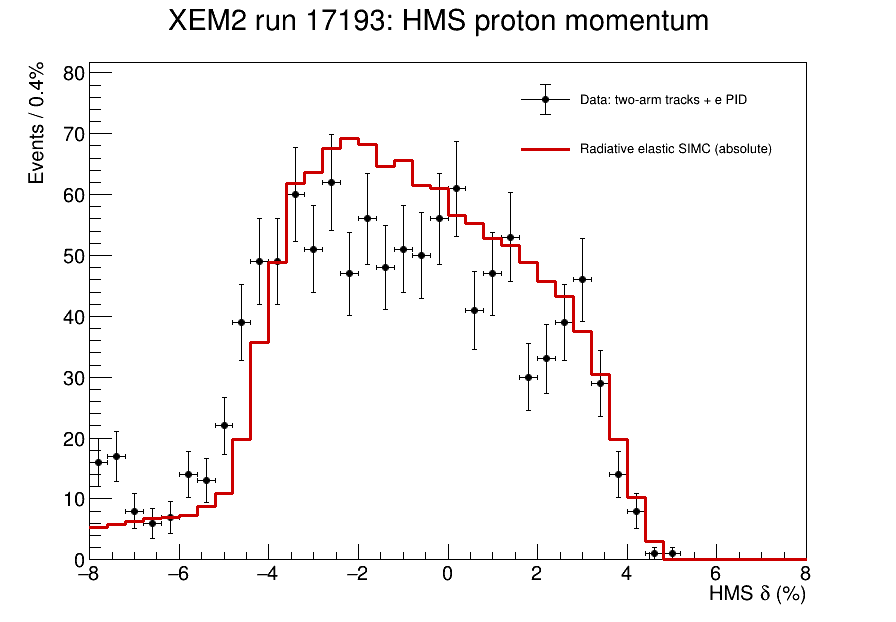
\includegraphics[width=\linewidth]{../plots/xem2_run17193_hms_dp_simc.png}
      \vspace{-0.2cm}
      {\scriptsize XEM2 run 17193: HMS $+6.476$ GeV/$c$ at $19.52^\circ$;
      proposed HMS $+6.735$ GeV/$c$ at $18.80^\circ$.}
    \column{0.46\textwidth}
      \begin{itemize}
        \item Broad HMS acceptance: data/SIMC $=0.936$.
        \item Tight elastic selection: $800/1034.34=0.7734$.
        \item At fixed 30 cm target length, NPS at 3 m gains a factor $4.11$
        over SHMS-like electron acceptance.
        \item Transfer from the XEM2 setting to \qval{}: SIMC ratio $=0.8865$.
        \item Direct \qval{} target scan: 20/10 cm $=1.85$ and
        30/10 cm $=2.57$; the final 10 cm supplies 28\% of the 30 cm yield.
      \end{itemize}

      \begin{block}{45 PAC-day projection}
        \begin{tabular}{@{}lr@{}}
          \toprule
          Before NPS response & \textbf{10.69 M} \\
          70\% threshold + fiducial & \textbf{7.70 M} \\
          80\% threshold + fiducial & \textbf{7.51 M} \\
          \bottomrule
        \end{tabular}
      \end{block}
      {\scriptsize Response values remain provisional (3$\times$3 energy,
      radiative photons, passive material). The sweeper will be absent in GEp;
      retaining it here is a small conservative effect.}
  \end{columns}
\end{frame}

% -----------------------------------------------------------------------------
\begin{frame}[shrink=18]{HMS trigger: the practical S1 rate is 40--60 kHz}
  \begin{columns}[T,onlytextwidth]
    \column{0.56\textwidth}
      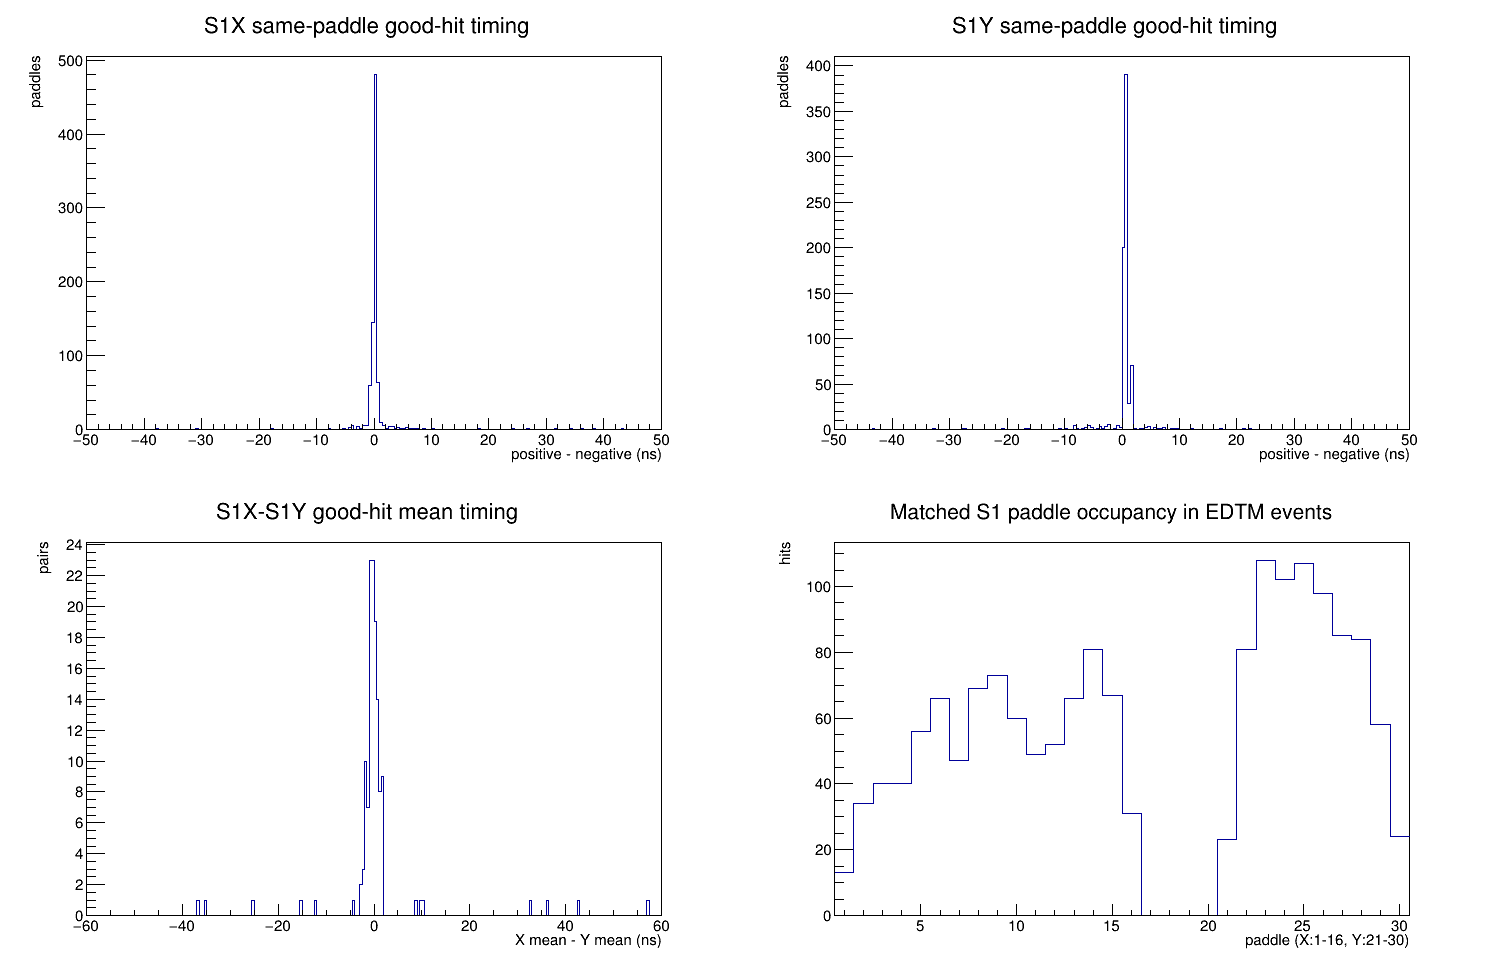
\includegraphics[width=\linewidth]{../plots/xem2_hms_paddle_good_edtm.png}
      \vspace{-0.15cm}
      {\scriptsize Run 17193 unbiased EDTM windows. A valid plane hit requires
      both PMTs on one physical paddle; valid X and Y paddle numbers are independent.}
    \column{0.42\textwidth}
      \begin{itemize}
        \item The branch previously labeled ``S1X AND S1Y'' is actually
        \textbf{S1X OR S1Y}; its GEp-scaled rate is about 810 kHz.
        \item EDTM plane rates reproduce direct scalers to 3--4\%.
        \item Requiring a double-ended paddle hit in both planes gives
        12.73--14.84 kHz at the run conditions.
        \item Naive GEp scaling gives \alert{51--60 kHz}; scaler
        inclusion--exclusion gives 39.9 kHz.
        \item HMS 3-of-4 scales to about \textbf{2.9 kHz} if it is compatible
        with the FPP configuration.
      \end{itemize}

      \begin{block}{Accidental scale}
        For 50 kHz HMS and 1 MHz NPS:
        \[R_{\rm acc}=R_HR_N\Delta t =
        \begin{cases}1~\mathrm{kHz},&20~\mathrm{ns}\\2~\mathrm{kHz},&40~\mathrm{ns}.\end{cases}\]
      \end{block}
  \end{columns}
\end{frame}

% -----------------------------------------------------------------------------
\begin{frame}[shrink=10]{NPS singles: the inclusive-electron component is data anchored}
  \begin{columns}[T,onlytextwidth]
    \column{0.57\textwidth}
      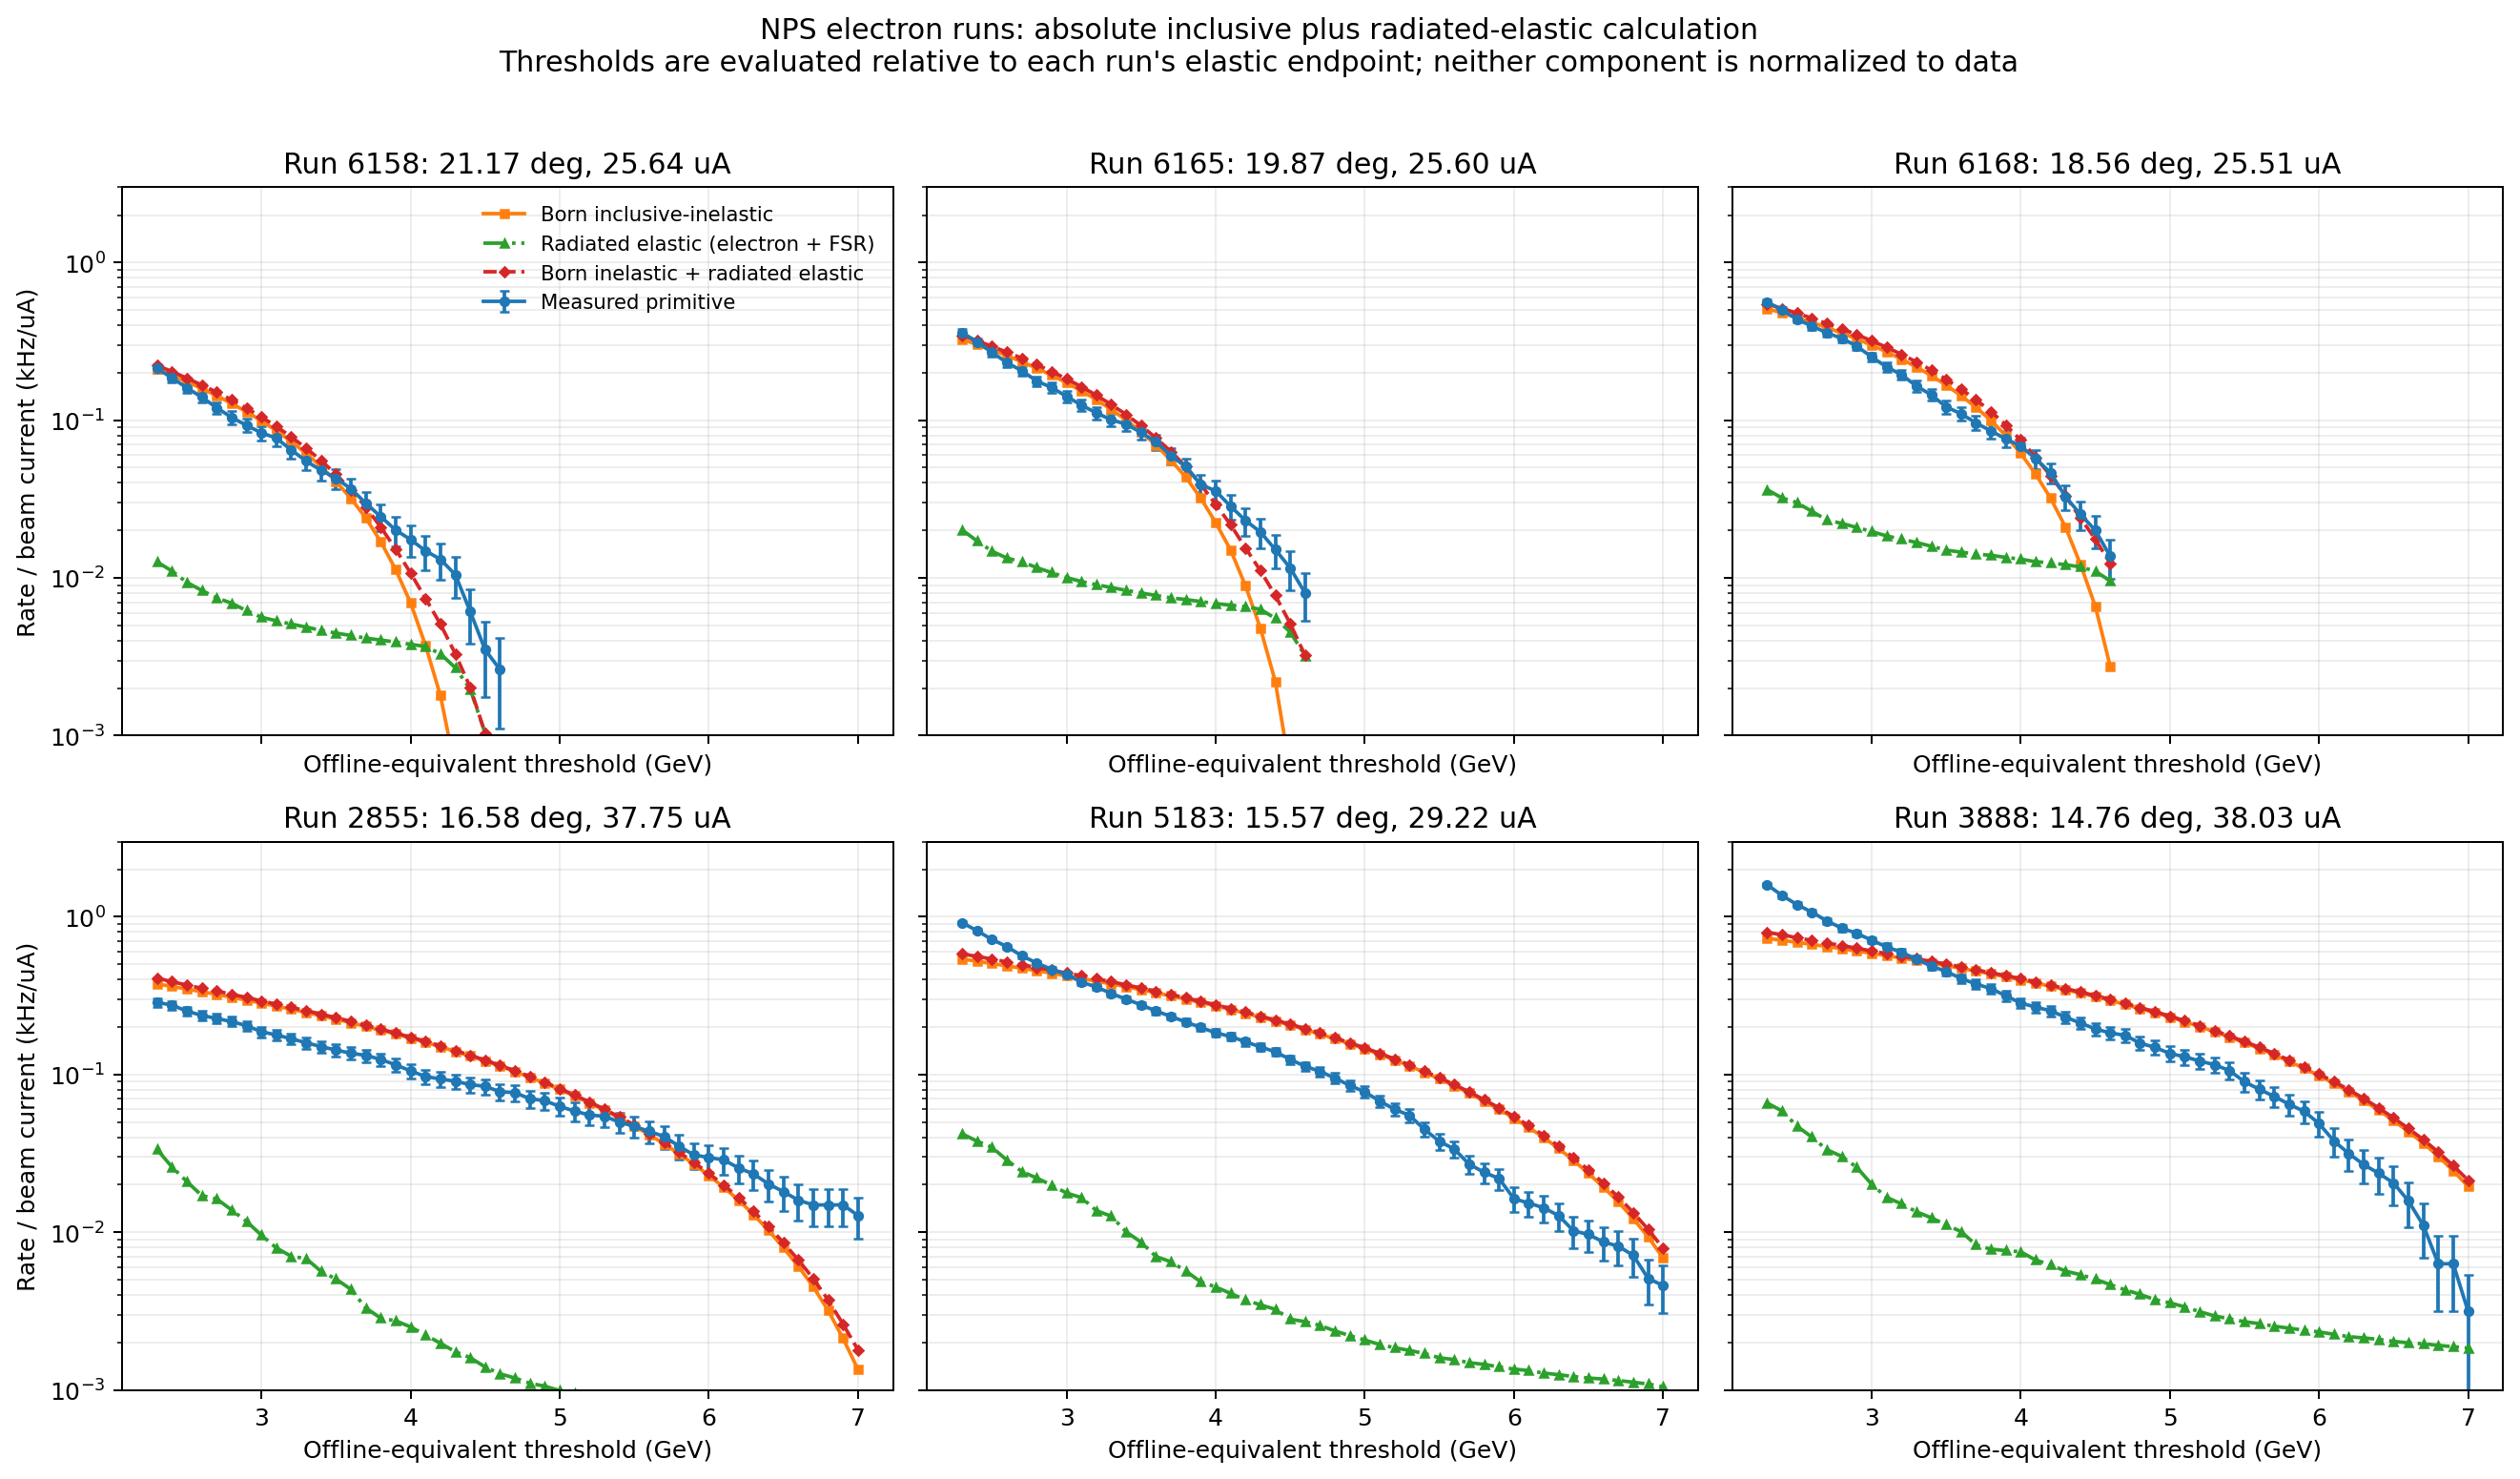
\includegraphics[width=\linewidth]{../plots/nps_inclusive_generator_six_run_validation.png}
    \column{0.41\textwidth}
      \begin{itemize}
        \item Three-pass NPS electron data: generator/data $=0.95$--$1.35$.
        \item Five-pass NPS electron data: trend reproduced; most discrepancies
        are conservative overpredictions.
        \item XEM2 SHMS electron-enriched trigger: 447.7 Hz predicted versus
        592 Hz measured, or 74.8\%.
      \end{itemize}

      \begin{block}{GEp full-face prediction}
        \centering
        \begin{tabular}{ccc}
          \toprule
          Threshold & Inclusive $e^-$ & + radiated elastic \\
          \midrule
          70\% & 14.34 kHz & \textbf{14.42 kHz} \\
          75\% & 10.26 kHz & \textbf{10.30 kHz} \\
          80\% & 7.05 kHz & \textbf{7.08 kHz} \\
          \bottomrule
        \end{tabular}
      \end{block}
      {\small\alert{These are genuine-electron rates, not the total NPS trigger rate.}}
  \end{columns}
\end{frame}

% -----------------------------------------------------------------------------
\begin{frame}{Run 6887 establishes a large non-electron excess}
  \begin{center}
    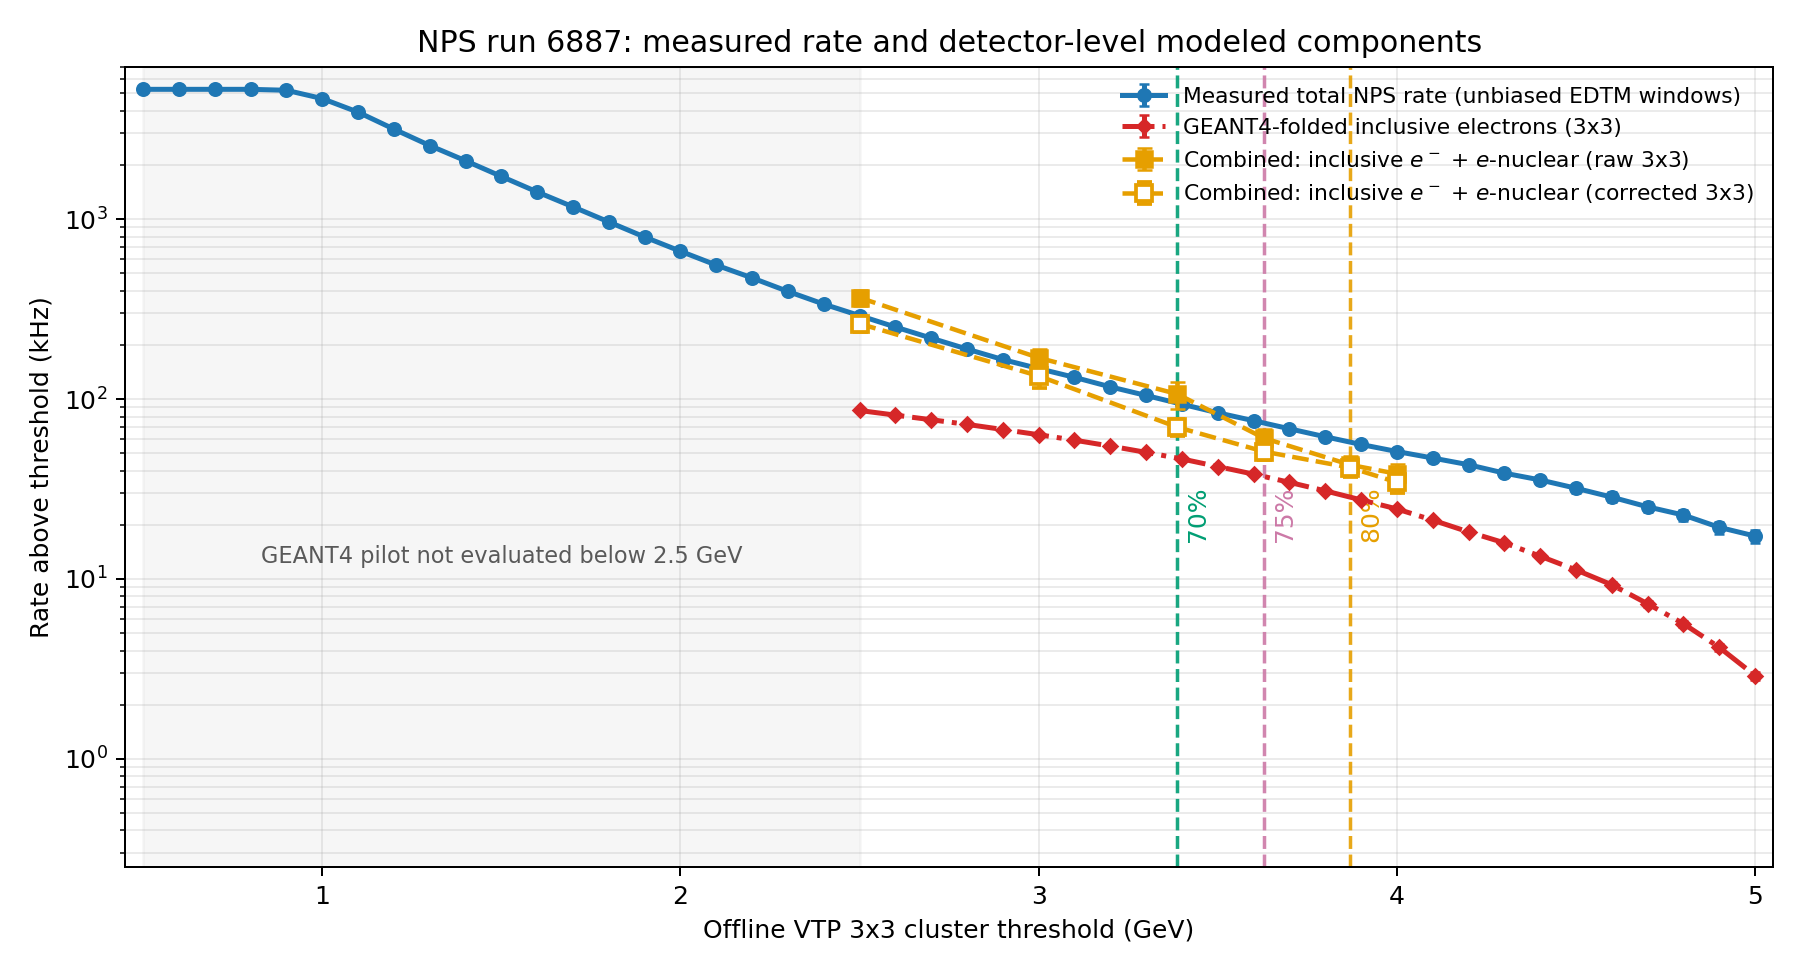
\includegraphics[width=0.53\linewidth]{../trigger_particle_composition/nps_run6887_measured_vs_geant4_electrons_slide.png}
  \end{center}
  \vspace{-0.27cm}
  \begin{center}
    \scriptsize
    \textbf{Run 6887:} DVCS production, NPS on the photon arm; 8.456 GeV beam,
    29.4 $\mu$A, 10 cm LH$_2$; NPS at $16.57^\circ$ and 3.57 m.\\[-0.02cm]
    VTP single-cluster trigger/readout settings: 0.50/0.25 GeV; 8,972 unbiased
    1-$\mu$s EDTM windows after the 25--35 $\mu$A current selection.
  \end{center}
  \vspace{-0.18cm}
  \begin{block}{What the data establish}
    \scriptsize
    At 70--80\%, inclusive electrons alone explain only 25--50\% of the rate.
    Adding importance-sampled electronuclear production gives 107, 61, and
    43 kHz with raw 3x3 energy, or 70, 51, and 42 kHz with the inherited
    correction.  The six direct points use the 0.25-GeV production cut.
    \textbf{The background is now at the required scale}; the high-threshold
    deficit and 3x3 energy convention remain open.
  \end{block}
\end{frame}

% -----------------------------------------------------------------------------
\begin{frame}{A single analyzer preserves the small-angle FPP acceptance}
  \begin{columns}[T,onlytextwidth]
    \column{0.50\textwidth}
      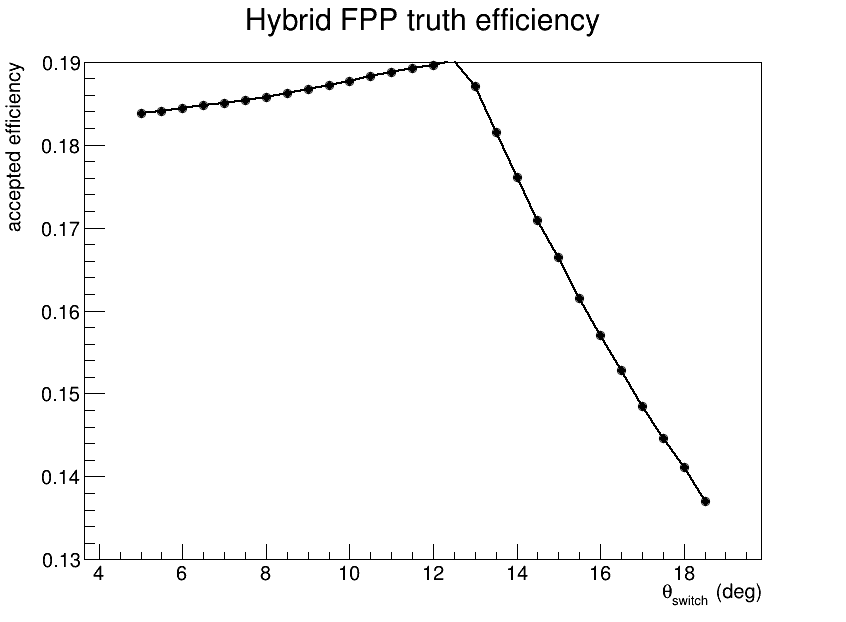
\includegraphics[width=\linewidth]{figures/single_55p88cm_hybrid_theta_switch.png}

    \column{0.48\textwidth}
      \small
      \begin{itemize}
        \item Legacy FPP frame: one 22-inch CH$_2$ analyzer.
        \item $\theta_{\rm polar}<12^\circ$: reconstruct with FPP1--FPP4;
        four chambers constrain the left/right ambiguity.
        \item $\theta_{\rm polar}>12^\circ$: reconstruct with FPP1 and FPP2;
        the larger deflection resolves the ambiguity and avoids downstream
        cone-test loss.
        \item Truth efficiency peaks near the
        \alert{$12^\circ$ transition}.
      \end{itemize}

      \begin{block}{Four-chamber closure}
        All 59,113 truth-selected events from $0^\circ$ to $10^\circ$
        reconstruct in the ideal fit, with no large angular outliers.
      \end{block}
  \end{columns}

  \vspace{-0.04cm}
  {\tiny\alert{Ideal closure:} truth-associated hits and exact drifts;
  efficiency, resolution, noise, and pattern recognition remain.}
\end{frame}

% -----------------------------------------------------------------------------
\begin{frame}{Hall C chamber geometry and wire-level tracking}
  \begin{columns}[T,onlytextwidth]
    \column{0.34\textwidth}
      \centering
      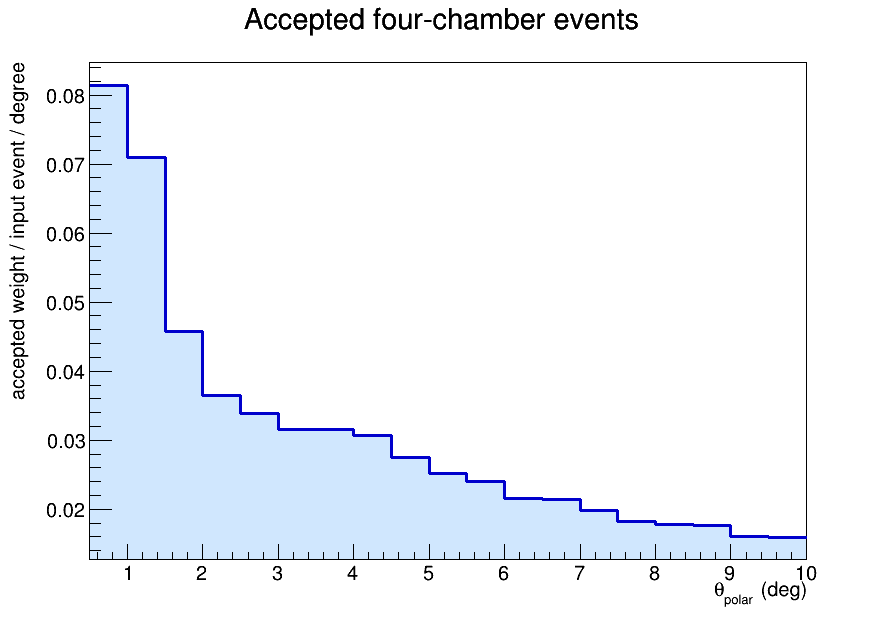
\includegraphics[width=\linewidth]{figures/single_55p88cm_accepted_efficiency_0_10deg.png}
    \column{0.33\textwidth}
      \centering
      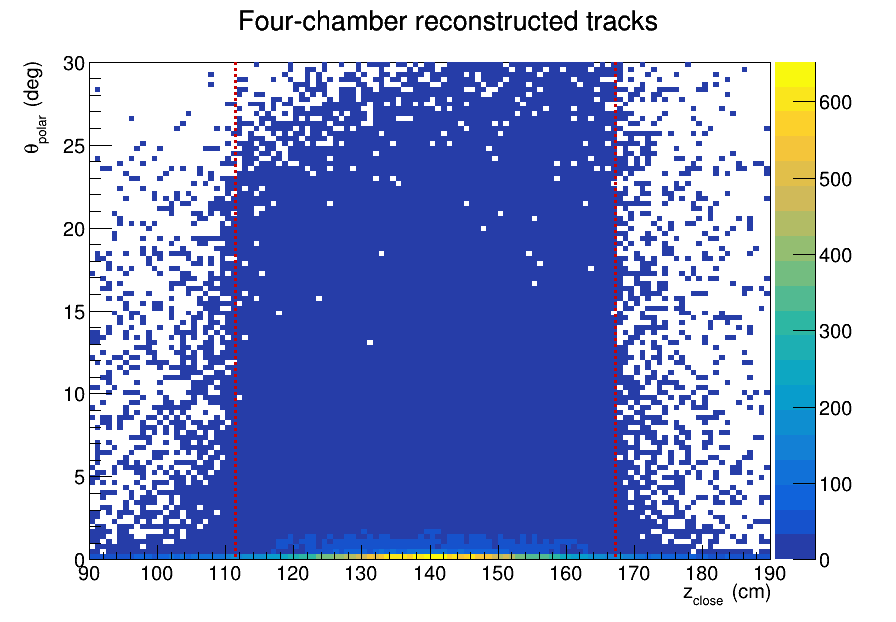
\includegraphics[width=\linewidth]{figures/single_55p88cm_theta_zclose.png}
    \column{0.33\textwidth}
      \centering
      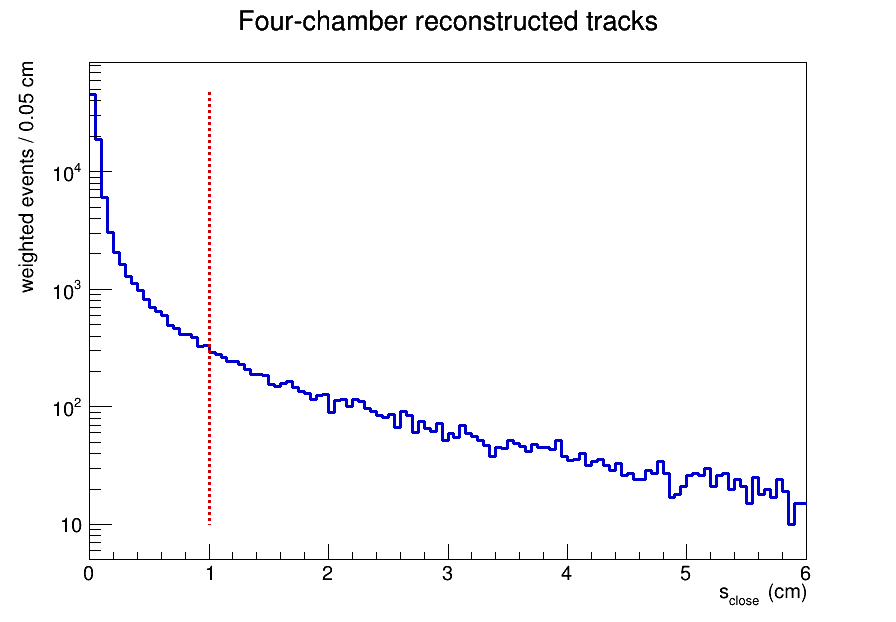
\includegraphics[width=\linewidth]{figures/single_55p88cm_sclose.png}
  \end{columns}

  \vspace{-0.12cm}
  {\scriptsize
  \begin{itemize}
    \item Ported the four measured chamber positions and twelve U/X/V planes
    from the GEp-III parameters: 104/83/104 wires per chamber with 2 cm pitch.
    \item Digitize plane and wire number plus unsigned drift distance; enumerate
    the left/right signs and retain the minimum reduced-$\chi^2$ $x(z),y(z)$ fit.
    \item Calculate the FPP observables relative to the HMS track and apply the
    cone test.  The efficiency density at left includes the analyzer-volume,
    cone-test and 1 cm $s_{\rm close}$ requirements on truth-associated candidates.
  \end{itemize}}

  \vspace{-0.02cm}
  {\tiny\alert{Ideal closure:} truth-associated hits and exact drifts; the fit
  receives neither the truth coordinate nor its sign. Detector response and
  multi-track recognition remain.}
\end{frame}

% -----------------------------------------------------------------------------
\begin{frame}{Single-track vs. Multi-track FOM}
  \scriptsize
  Use the same beam-polarization-weighted normalization per incident proton:
  \[
    \mathrm{FOM}=P_e^2\,\epsilon_{\rm FPP}\langle A_y^2\rangle,
    \qquad P_e=0.85.
  \]
  \vspace{-0.25cm}
  \begin{center}
    \renewcommand{\arraystretch}{1.35}
    \begin{tabular}{@{}lccc@{}}
      \toprule
      Estimate / selection & Useful efficiency & $A_y$ input & FOM / proton \\
      \midrule
      Andrew's planning estimate & 20\% assumed & $\sim$0.050 & $\sim3.60\times10^{-4}$ \\
      Hall C: single tracks (no $1^\circ$ cut) & 12.492\% & 0.05859 RMS & $3.10\times10^{-4}$ \\
      Hall C: smallest angle $>1^\circ$ & 25.892\% & 0.06704 RMS & $8.41\times10^{-4}$\rlap{$^{*}$} \\
      \bottomrule
    \end{tabular}
  \end{center}
  \vspace{-0.1cm}
  \begin{block}{What explains the initial discrepancy}
    \small
    Our original $7.56\times10^{-4}$ included multi-track events.
    Restricting to single tracks gives a result only \textbf{14\% below Andrew's}
    $3.6\times10^{-4}$ estimate, with the GEp-III $A_y$ parametrization.
  \end{block}
  {\scriptsize Andrew uses an estimated average $A_y$; the simulation integrates
  $A_y^2$ event by event. FOM agreement does not imply identical efficiency or cuts.\\[2pt]
  $^{*}$Multi-track FOM is provisional: it assumes the single-track $A_y$ model applies.}
  \note{Andrew Puckett email to Ed Brash, 10 November 2026, 11:30 AM, pp. 2--3 of andrew.pdf.
  Andrew quotes 3.6e-4 per incident proton; 20 percent and Ay approximately 0.05 give
  0.20*(0.85*0.05)^2=3.6125e-4. Hall C numbers: comparison_gt1.json,
  run track_selection_14574698 in /work/hallc/gep/brash/gep4_fpp_geant4/runs.
  100,000 central-ray 6.7 GeV/c protons, FTFP_BERT, 55.88 cm CH2.
  Exclusive-single-track row retains the original useful-pT window without an explicit
  one-degree cut. Smallest-angle row restricts candidates to theta strictly above
  one degree before ranking. Both are ideal truth-associated selections.}
\end{frame}

% -----------------------------------------------------------------------------
\begin{frame}{Analyzing-power parametrization and FOM weighting}
  \small
  The same construction appears in the SBS planning code and Andrew's description:
  \[
    A_y(p,p_T)=\left(0.0342+\frac{0.348}{p}\right)
      \sqrt{2eb}\,p_Te^{-bp_T^2},
    \qquad b=2.42614689.
  \]
  {\scriptsize $b$: inverse-variance-weighted mean of the three high-$Q^2$ fits;
  $A_y^{\max}=0.0342+0.348/p$. Use $p_T=p\sin\theta$, with $p,p_T$ in GeV/$c$.}

  \vspace{0.12cm}
  \textbf{Same exclusive single-track sample:}
  $p=6.7$ GeV/$c$, $\epsilon=12.492\%$, $P_e=0.85$.
  \begin{center}
    \renewcommand{\arraystretch}{1.25}
    \begin{tabular}{@{}lcc@{}}
      \toprule
      Averaging convention & Effective $A_y$ & FOM / incident proton \\
      \midrule
      Square of mean: $P_e^2\epsilon\langle A_y\rangle^2$
        & 0.05484 & $2.714\times10^{-4}$ \\
      Mean square: $P_e^2\epsilon\langle A_y^2\rangle$
        & 0.05859 RMS & $3.099\times10^{-4}$ \\
      \bottomrule
    \end{tabular}
  \end{center}
  \vspace{-0.10cm}
  \textbf{Event-by-event weighting gives 14.2\% more FOM}, not a factor of two.
  No parametrization mismatch was found.

  \vspace{0.18cm}
  {\scriptsize Table VII's $\bar A_y$ is an asymmetry-calibrated effective average,
  not an RMS. Its $0.06\le p_T\le1.2$ GeV/$c$ range also differs from our
  $0.07\le p_T\le1.0$ GeV/$c$ selection (no explicit $1^\circ$ cut here).}
  \note{Sources: Puckett et al., Phys. Rev. C 96, 055203 (2017),
  Sec. III.B.7 and Table VII; https://arxiv.org/html/1707.08587 .
  Local primary code: /Users/brash/g4sbs/root_macros/GEP_FOM_quick_and_dirty.C,
  lines 95--131, 467--468 and 502--504. Our analysis/analyzing_power.py has
  identical constants and functional form. Numerical comparison at 1,407
  momentum/angle combinations gave maximum relative discrepancy 9.5e-16.
  Andrew's current private source was not inspected; his email description
  and the locally available SBS macro match our implementation.
  b uses (2.376 +/- 0.189), (2.776 +/- 0.212), (2.292 +/- 0.145).
  At p=6.7 GeV/c the peak Ay is 0.0861403, at pT=0.453969 GeV/c,
  theta=3.88514 degrees; neither the mean nor RMS is the peak.
  Means were recomputed from the 12,492 useful single-track events in
  comparison_gt1_events.csv from run track_selection_14574698.
  Mean Ay=0.054839906861449884; RMS Ay=0.058594874252813275.
  The FOM ratio is 1.141631218. This is a comparison of averaging conventions
  for identical simulated events, not a comparison of different acceptances.
  Full form-factor uncertainty still requires event-dependent spin transport.}
\end{frame}

% -----------------------------------------------------------------------------
\begin{frame}{SBS asymmetry supports the analyzing-power scale}
  \small
  Andrew's preliminary $Q^2=11$ GeV$^2$ data give a sine amplitude
  $|s|=0.02971\pm0.00403$. In the leading dipole approximation,
  \[
    A_{y,\mathrm{eff}}\simeq
      \frac{|s|}{P_eP_\ell|\sin\chi|},
    \qquad P_e\simeq0.87.
  \]
  {\scriptsize Illustrative Born kinematics: $E=10.7$ GeV,
  $Q^2=11$ GeV$^2$, $\mu_pG_E/G_M=0.2$ give $\epsilon=0.684$,
  $P_\ell=0.729$, $P_t=-0.027$ for a fully polarized beam.}

  \vspace{0.12cm}
  \begin{center}
    \renewcommand{\arraystretch}{1.25}
    \begin{tabular}{@{}lc@{}}
      \toprule
      Estimate / assumption & Effective average $A_y$ \\
      \midrule
      SBS data, $|\sin\chi|=1$ & $0.0468\pm0.0064$ \\
      SBS data, $\chi=1.3$ rad & $0.0486\pm0.0066$ \\
      Our simulated single-track mean & 0.05484 \\
      \bottomrule
    \end{tabular}
  \end{center}
  \vspace{-0.10cm}
  \textbf{The estimates agree within roughly one statistical standard deviation.}
  Varying $\mu_pG_E/G_M$ from 0 to 0.4 changes $P_\ell$ by less than 0.5\%.

  \vspace{0.15cm}
  {\scriptsize Errors shown propagate the plotted asymmetry uncertainty only.
  This estimate uses approximate central kinematics and spin precession;
  acceptance averaging and background dilution are not determined here.
  It estimates a mean $A_y$, not the RMS, and does not validate multi-track FOM.\\[2pt]
  Source: A. Puckett, SBS Collaboration Meeting, 2 March 2026, slides 9, 10, 36.}
  \note{Primary source: Andrew Puckett, GEP Analysis Status, 2 March 2026,
  https://indico.jlab.org/event/1009/contributions/18155/attachments/13773/22270/PuckettGEP.pdf .
  Slide 36 data fit: c1=0.001119 +/- 0.003662, s1=-0.02971 +/- 0.00403;
  simulated fit: c1=0.004153 +/- 0.002613, s1=-0.03147 +/- 0.00261.
  Absolute sine amplitudes are used to avoid coordinate-sign ambiguity.
  Data/simulation sine-amplitude ratio=0.944 +/- 0.150, assuming independent
  fit errors; its interpretation as an Ay scale ratio additionally assumes
  matching beam polarization, spin transport, and accepted kinematics.
  Slide 9 locates the SBS high-Q2 precession near maximal longitudinal-to-
  transverse conversion; chi=1.3 rad is illustrative, not a measured mean.
  Slide 10 gives approximate beam polarization of 87 percent.
  Born polarization formulas: Puckett et al., Phys. Rev. C 96, 055203 (2017),
  Sec. III.B.7, https://arxiv.org/html/1707.08587 .
  With epsilon=0.6836690815 and tau=3.1237416342, R=0.2 gives
  Pl=0.7289739740, Pt=-0.0266174758. Pl is normalized to Pe=1, so Pe enters
  the asymmetry conversion once. R=0--0.4 gives Pl=0.729792--0.726530.
  The comparison value 0.0548399069 is our ordinary single-track mean, not
  our RMS 0.0585948743. Different experimental and simulated acceptances
  prevent interpreting this rough consistency check as a calibrated extraction.}
\end{frame}

% -----------------------------------------------------------------------------
\begin{frame}{SBS detailed yield accounting}
  \small
  Andrew's reconstruction study supplies the missing definition of the SBS
  ``best case'' sample:
  \[
    \underbrace{12\ \mathrm{M}}_{\substack{\mathrm{digi+recon,\ trigger,}\
      \mathrm{exclusivity,\ FT/FPP\ tracks}}}
    \times\underbrace{0.70}_{\mathrm{global\ performance}}
    \simeq\underbrace{9\ \mathrm{M}}_{\mathrm{selected}}
    \times\underbrace{0.33}_{\mathrm{useful\ polarimetry}}
    \simeq\underbrace{2.9\ \mathrm{M}}_{\mathrm{useful\ events}}.
  \]

  \begin{center}
    \renewcommand{\arraystretch}{1.22}
    \begin{tabular}{@{}lcc@{}}
      \toprule
      SBS estimate & Useful events & Projected $\sigma(\mu_pG_E/G_M)$ \\
      \midrule
      Andrew's stated quick-spreadsheet estimate & 5.1 M & $\simeq0.10$ \\
      Detailed reconstruction and cuts & 2.9 M & $\simeq0.13$ \\
      \bottomrule
    \end{tabular}
  \end{center}
  \vspace{-0.08cm}
  The uncertainty follows the expected count scaling:
  $0.10\sqrt{5.1/2.9}=0.133$.

  \vspace{0.12cm}
  {\scriptsize The 2.9 M count already includes the useful-polarimetry fraction;
  another 20\% or 33\% efficiency would double count it. The SBS generator is
  Born-only, so Andrew estimates that the useful yield remains 10--15\% high.}
  \note{Primary source: Andrew Puckett email to Ed Brash, 10 November 2026,
  page 5 of gep_hallc_reboot/andrew.pdf. Andrew states that the g4sbs sample
  passes digitization and reconstruction, ECAL and HCAL trigger-like cuts,
  dx, dy, and dpp exclusivity cuts, FT and FPP track requirements, and
  FPP sclose below 3 mm. About 12 million events pass before the 70 percent
  global factor. The useful-polarimetry fraction relative to the resulting
  approximately 9 million events is about 33 percent, giving 2.9 million.
  His quick spreadsheet uses 5.1 million useful events and projects about
  0.10 absolute statistical uncertainty in mu_p GE/GM. He obtains about
  0.13 after naive square-root count scaling. The detailed SBS generator is
  Born-only; Andrew estimates a further 10--15 percent yield reduction when
  comparing with the fully radiated Hall C SIMC calculation.}
\end{frame}

% -----------------------------------------------------------------------------
\begin{frame}{Hall C and SBS FOM on a common basis}
  \small
  Using Andrew's $A_y=0.05$ and $P_e=0.85$, the detailed SBS sample gives
  \[
    \mathrm{FOM}_{\rm SBS}=2.9\times10^6(0.85\times0.05)^2=5238.
  \]
  \begin{center}
    \renewcommand{\arraystretch}{1.20}
    \begin{tabular}{@{}lcc@{}}
      \toprule
      Scenario & Total polarized FOM & $\sigma_{\rm component}$ \\
      \midrule
      SBS detailed, Born yield & 5,238 & 0.0195 \\
      SBS with 10--15\% radiative reduction & 4,452--4,714 & 0.0212--0.0206 \\
      Hall C, exclusive single track & 2,324--2,386 & 0.0293--0.0290 \\
      Hall C, smallest angle $>1^\circ$ & 6,306--6,474 & 0.0178--0.0176$^{*}$ \\
      \bottomrule
    \end{tabular}
  \end{center}
  \vspace{-0.08cm}
  {\scriptsize $^{*}$The Hall C multi-track result remains provisional. It applies the
  GEp-III single-track $A_y$ model to ideal truth-associated multi-track events.}

  \vspace{0.12cm}
  \begin{block}{Resolution of question 3}
    The former quick SBS construction gave nearly the correct aggregate FOM,
    but Andrew's 2.9 M ledger supplies the defensible interpretation. Hall C
    becomes modestly stronger only if useful multi-track events survive realistic
    reconstruction and retain the assumed analyzing power.
  \end{block}
  {\scriptsize Component errors are comparable feasibility metrics. A Hall C
  form-factor-ratio uncertainty still requires event-by-event spin transport
  and the polarization covariance.}
  \note{SBS calculations: 2.9e6*(0.85*0.05)^2=5238.125 and
  sigma_component=sqrt(2/FOM)=0.0195401. Reducing the SBS useful count by
  10 percent gives FOM=4714.31 and sigma=0.0205971; reducing by 15 percent
  gives FOM=4452.41 and sigma=0.0211942. Hall C uses N=7.5--7.7 million
  incident protons after the provisional NPS response. Exclusive-single-track
  polarized FOM per incident proton is 0.0003098768126. Smallest-angle-above-
  one-degree polarized FOM is 0.0008407773650. The older slide construction,
  9.3 million times 20 percent times (0.85*0.06311)^2, gave total FOM near
  5350, numerically close to Andrew's detailed 5238 despite different factors.
  Do not identify sigma_component with sigma(mu_p GE/GM).}
\end{frame}

% -----------------------------------------------------------------------------
\begin{frame}{Smallest-angle selection recovers useful multi-track events}
  \begin{center}
    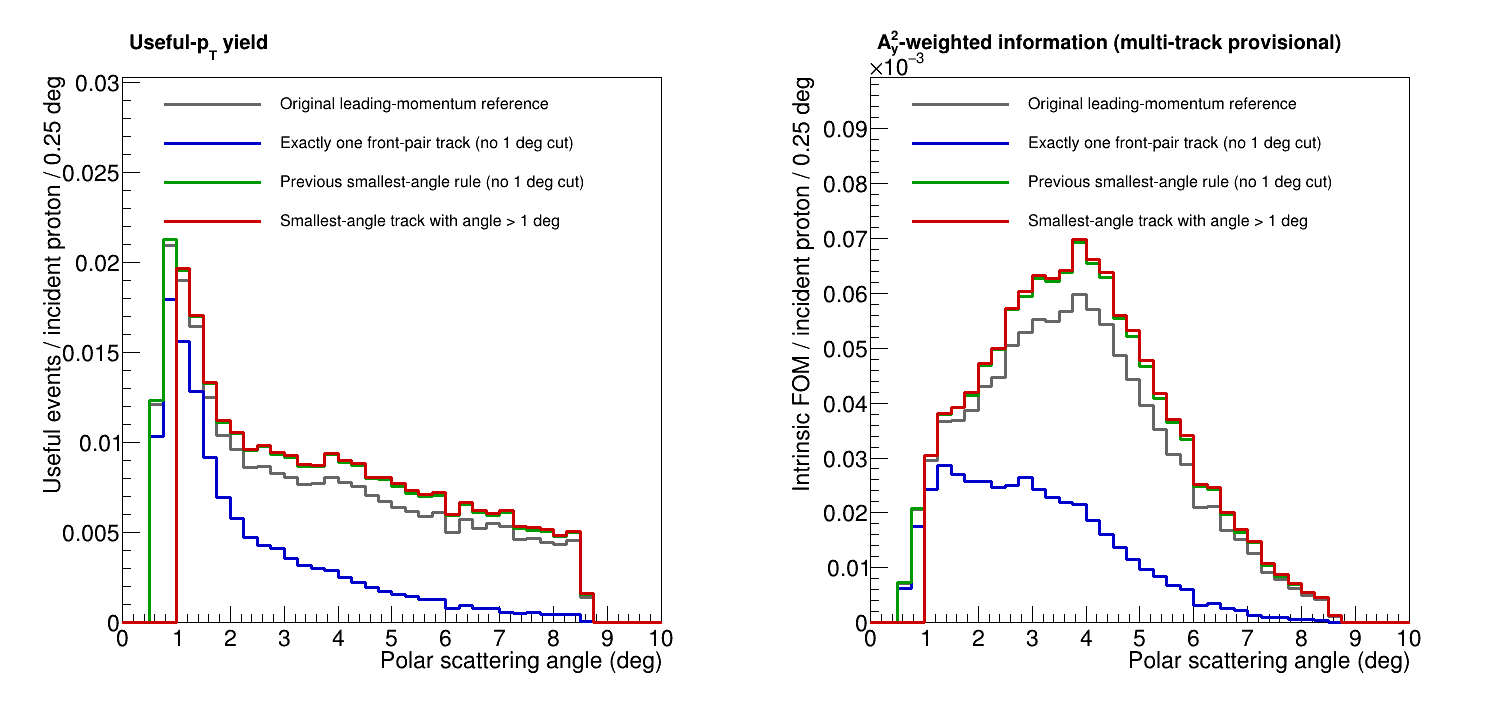
\includegraphics[width=0.98\linewidth,height=0.68\textheight,keepaspectratio]{figures/fpp_track_selection_gt1_2026-11-10.png}
  \end{center}
  \vspace{-0.20cm}
  {\scriptsize
  \textbf{Rule:} choose the smallest polar angle strictly above $1^\circ$, then
  apply the existing chamber, cone, closest-approach, and useful-$p_T$ cuts.\\[2pt]
  \textbf{Result:} 25,892 useful events, including 16,229 multi-track events,
  per 100,000 protons; 98.79\% of the previous FOM retained.}
  \note{Plot: comparison_gt1.png, generated from the same saved 100,000-event
  transport file used in the prior study; output provenance in comparison_gt1.json.
  All tracks crossing FPP1--FPP2 are counted before cuts. The chosen track must
  also cross FPP3--FPP4 below 12 degrees. The angle filter precedes ranking;
  a track at or below one degree does not veto another eligible track.
  No outgoing momentum is used in this choice. A chosen track that fails a
  remaining cut is not replaced. The exclusive-single-track blue reference
  retains no explicit one-degree bound; it is labeled accordingly in the plot.}
\end{frame}

% -----------------------------------------------------------------------------
\begin{frame}{Multi-track recovery could improve the FPP statistical reach}
  \small
  The single-track calculation supports Andrew's FOM scale. The simulation
  suggests that retaining some multi-track events could do better.
  \[
    \sigma_{\rm component}=\sqrt{\frac{2}{N\,\mathrm{FOM}}},
    \qquad N=7.5\text{--}7.7\times10^6.
  \]
  \begin{center}
    \renewcommand{\arraystretch}{1.25}
    \begin{tabular}{@{}lcc@{}}
      \toprule
      FPP selection & FOM / incident proton & $\sigma_{\rm component}$ \\
      \midrule
      Exclusive single tracks & $3.10\times10^{-4}$ & 0.0293--0.0290 \\
      Smallest angle $>1^\circ$, including multi-track & $8.41\times10^{-4}$ & 0.0178--0.0176\rlap{$^{*}$} \\
      \bottomrule
    \end{tabular}
  \end{center}
  \vspace{-0.10cm}
  {\scriptsize $^{*}$Provisional: GEp-III single-track $A_y$ applied to ideal,
  truth-associated multi-track events. Detector efficiency, resolution, noise,
  and multi-track pattern recognition remain to be included. These are
  polarization-component uncertainties, not uncertainties in $\mu_pG_E/G_M$.}
  \note{N=7.5--7.7 million is the pre-existing provisional Hall C elastic yield
  after NPS response, not a new yield determination. Component uncertainties
  use Pe=0.85 exactly once through polarized_fom. Full values for single tracks:
  FOM=0.00030987681259410263. For smallest angle strictly above one degree:
  FOM=0.0008407773650280434. Multiple-track analyzing power is not validated.
  Treat the single-track result as the baseline and multi-track recovery
  as a potential improvement.}
\end{frame}

% -----------------------------------------------------------------------------
\begin{frame}{Selected-track yield per incident proton}
  \begin{columns}[T,onlytextwidth]
    \begin{column}{0.53\textwidth}
      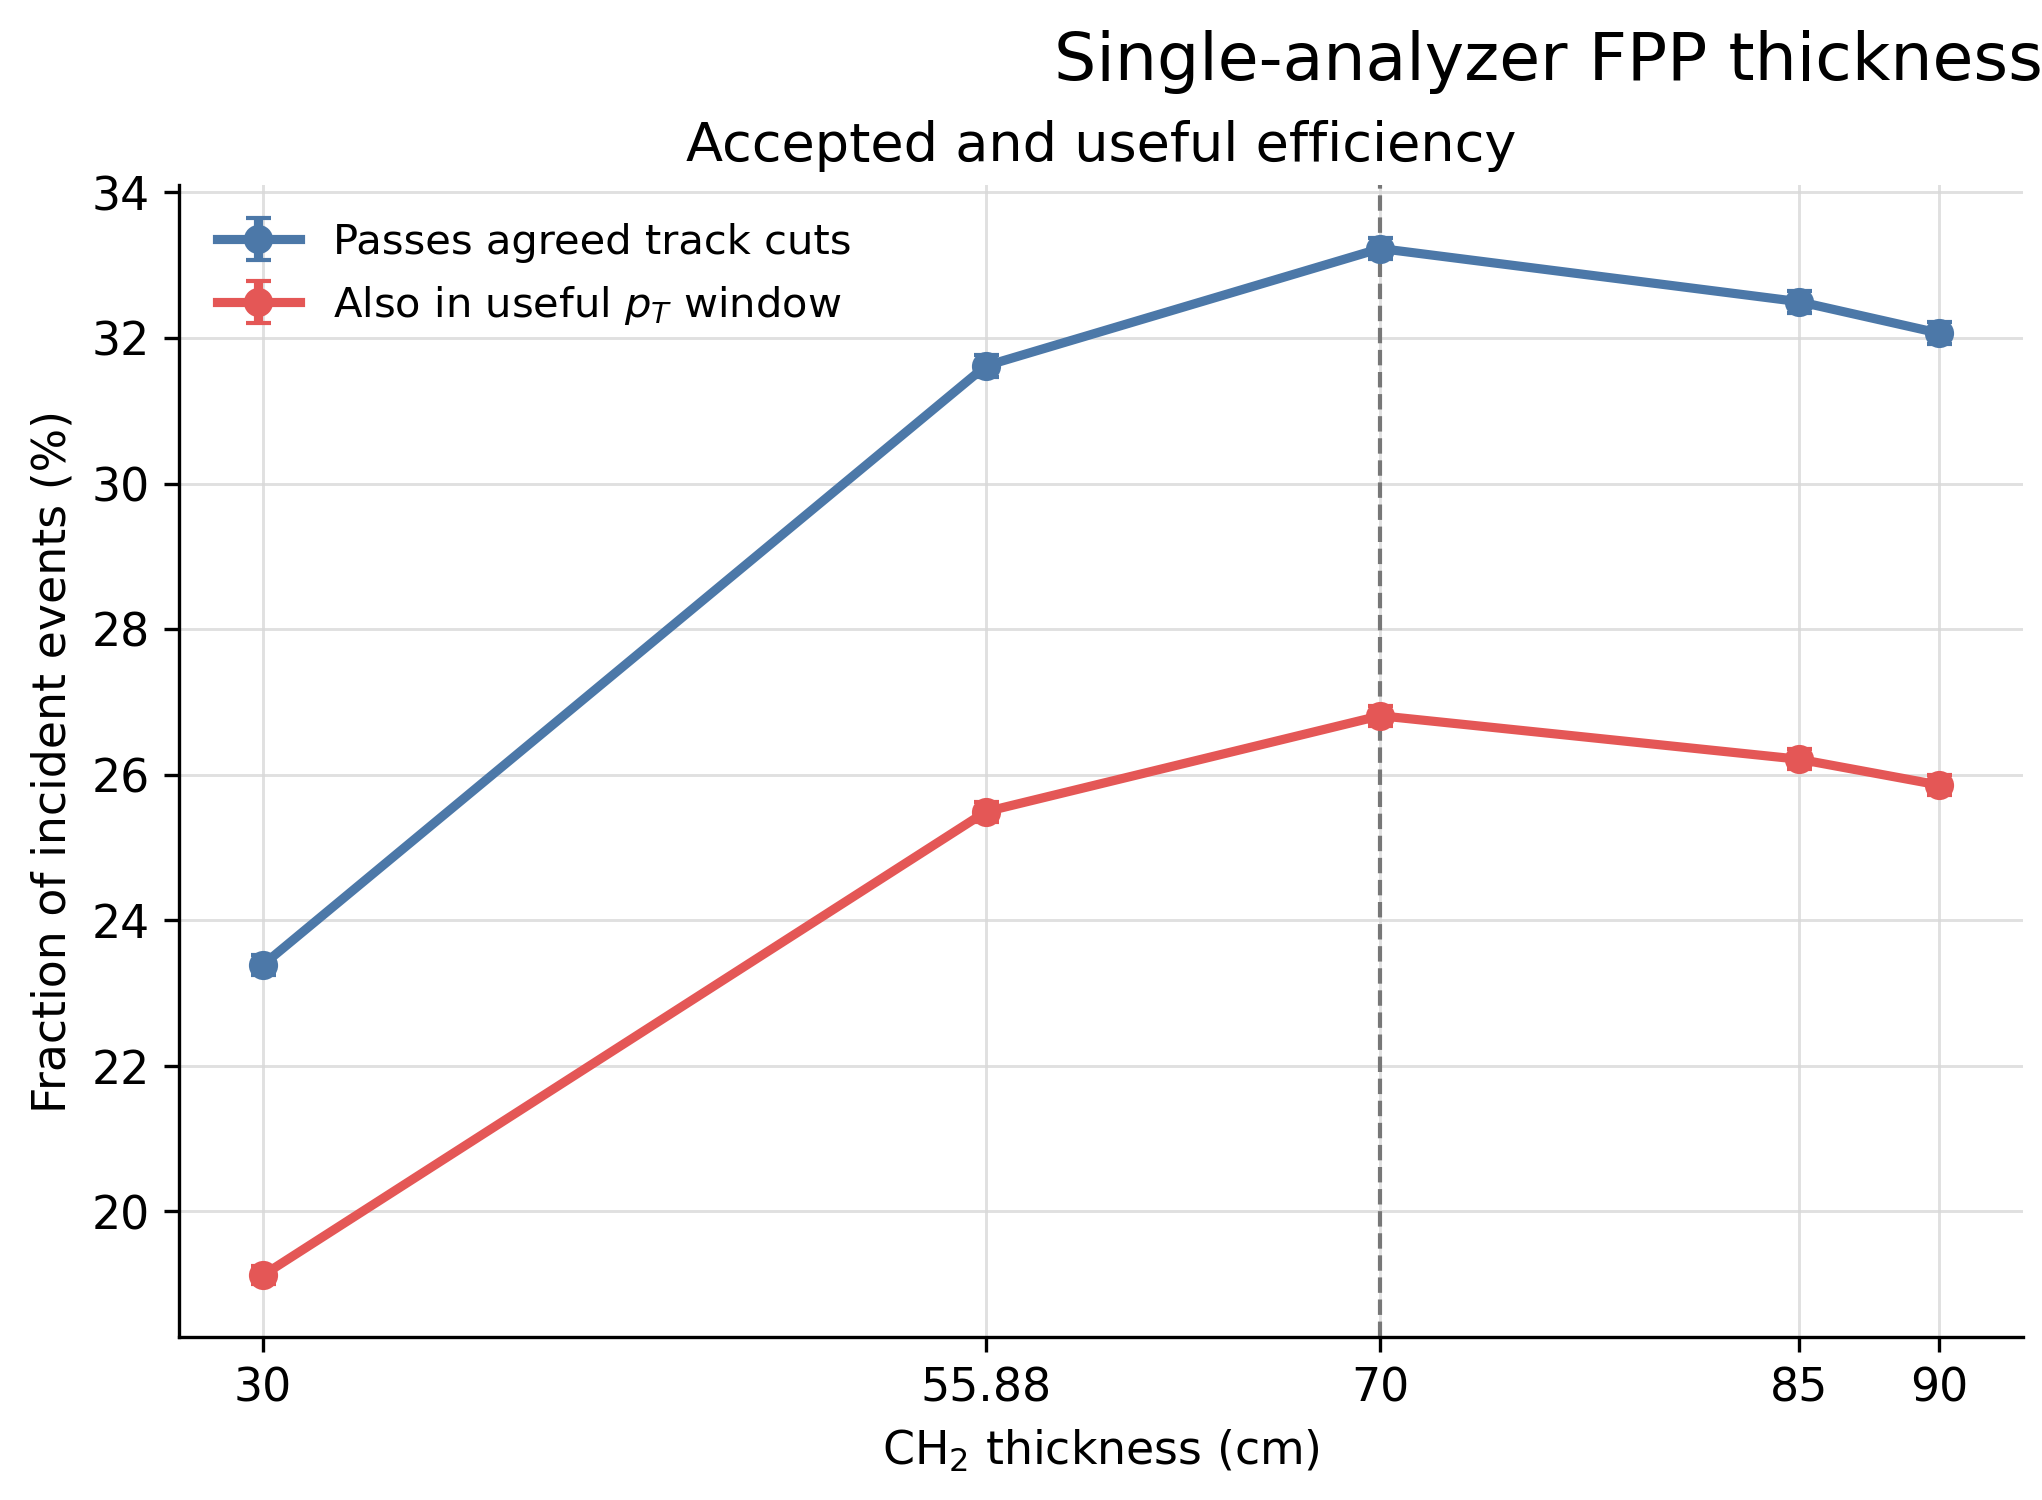
\includegraphics[width=\linewidth,height=0.56\textheight,keepaspectratio]{figures/thickness_efficiency_panel_corrected.png}
    \end{column}
    \begin{column}{0.45\textwidth}
      \scriptsize
      \begin{block}{Denominator for every point}
        100,000 unit-weight, 6.7 GeV/$c$ protons incident on the analyzer.
      \end{block}
      \textcolor{blue}{\textbf{Blue numerator: passes the agreed track cuts}}
      \begin{itemize}
        \item Among charged tracks crossing FPP1 and FPP2, retain angles
          strictly above $1^\circ$ and choose the smallest angle.
        \item Require that chosen track to cross all four chambers and pass
          the all-four cone test, $z_{\rm close}$ inside CH$_2$, and
          $s_{\rm close}\le1$ cm.
        \item If it fails, do not replace it with another track. Outgoing
          momentum never enters the choice.
      \end{itemize}
      \textcolor{red}{\textbf{Red numerator: useful-$p_T$ events}}
      \begin{itemize}
        \item Start with the blue events and require
          $0.07\le p_{\rm inc}\sin\theta\le1.00$ GeV/$c$, with
          $p_{\rm inc}=6.7$ GeV/$c$.
        \item The selected track may be the primary proton or a charged secondary.
      \end{itemize}
    \end{column}
  \end{columns}
  \vspace{-0.12cm}
  {\scriptsize
  \textbf{70 cm example:} Blue: $33{,}229/100{,}000=33.229\%$; red:
  $26{,}810/100{,}000=26.810\%$.\\
  The conditional ratio $26{,}810/33{,}229=80.68\%$ is not plotted.}
  \note{Both plotted quantities are absolute efficiencies per incident proton,
  not efficiencies conditional on passing the agreed track cuts. This analysis
  uses the same smallest-angle-strictly-above-one-degree policy as slide 15.
  The 55.88 cm result independently reproduces the slide-15 workflow:
  useful efficiency 0.25492 and intrinsic FOM 0.00114463792389906.}
\end{frame}

% -----------------------------------------------------------------------------
\begin{frame}{Charged-track multiplicity before analysis cuts}
  \begin{columns}[T,onlytextwidth]
    \begin{column}{0.56\textwidth}
      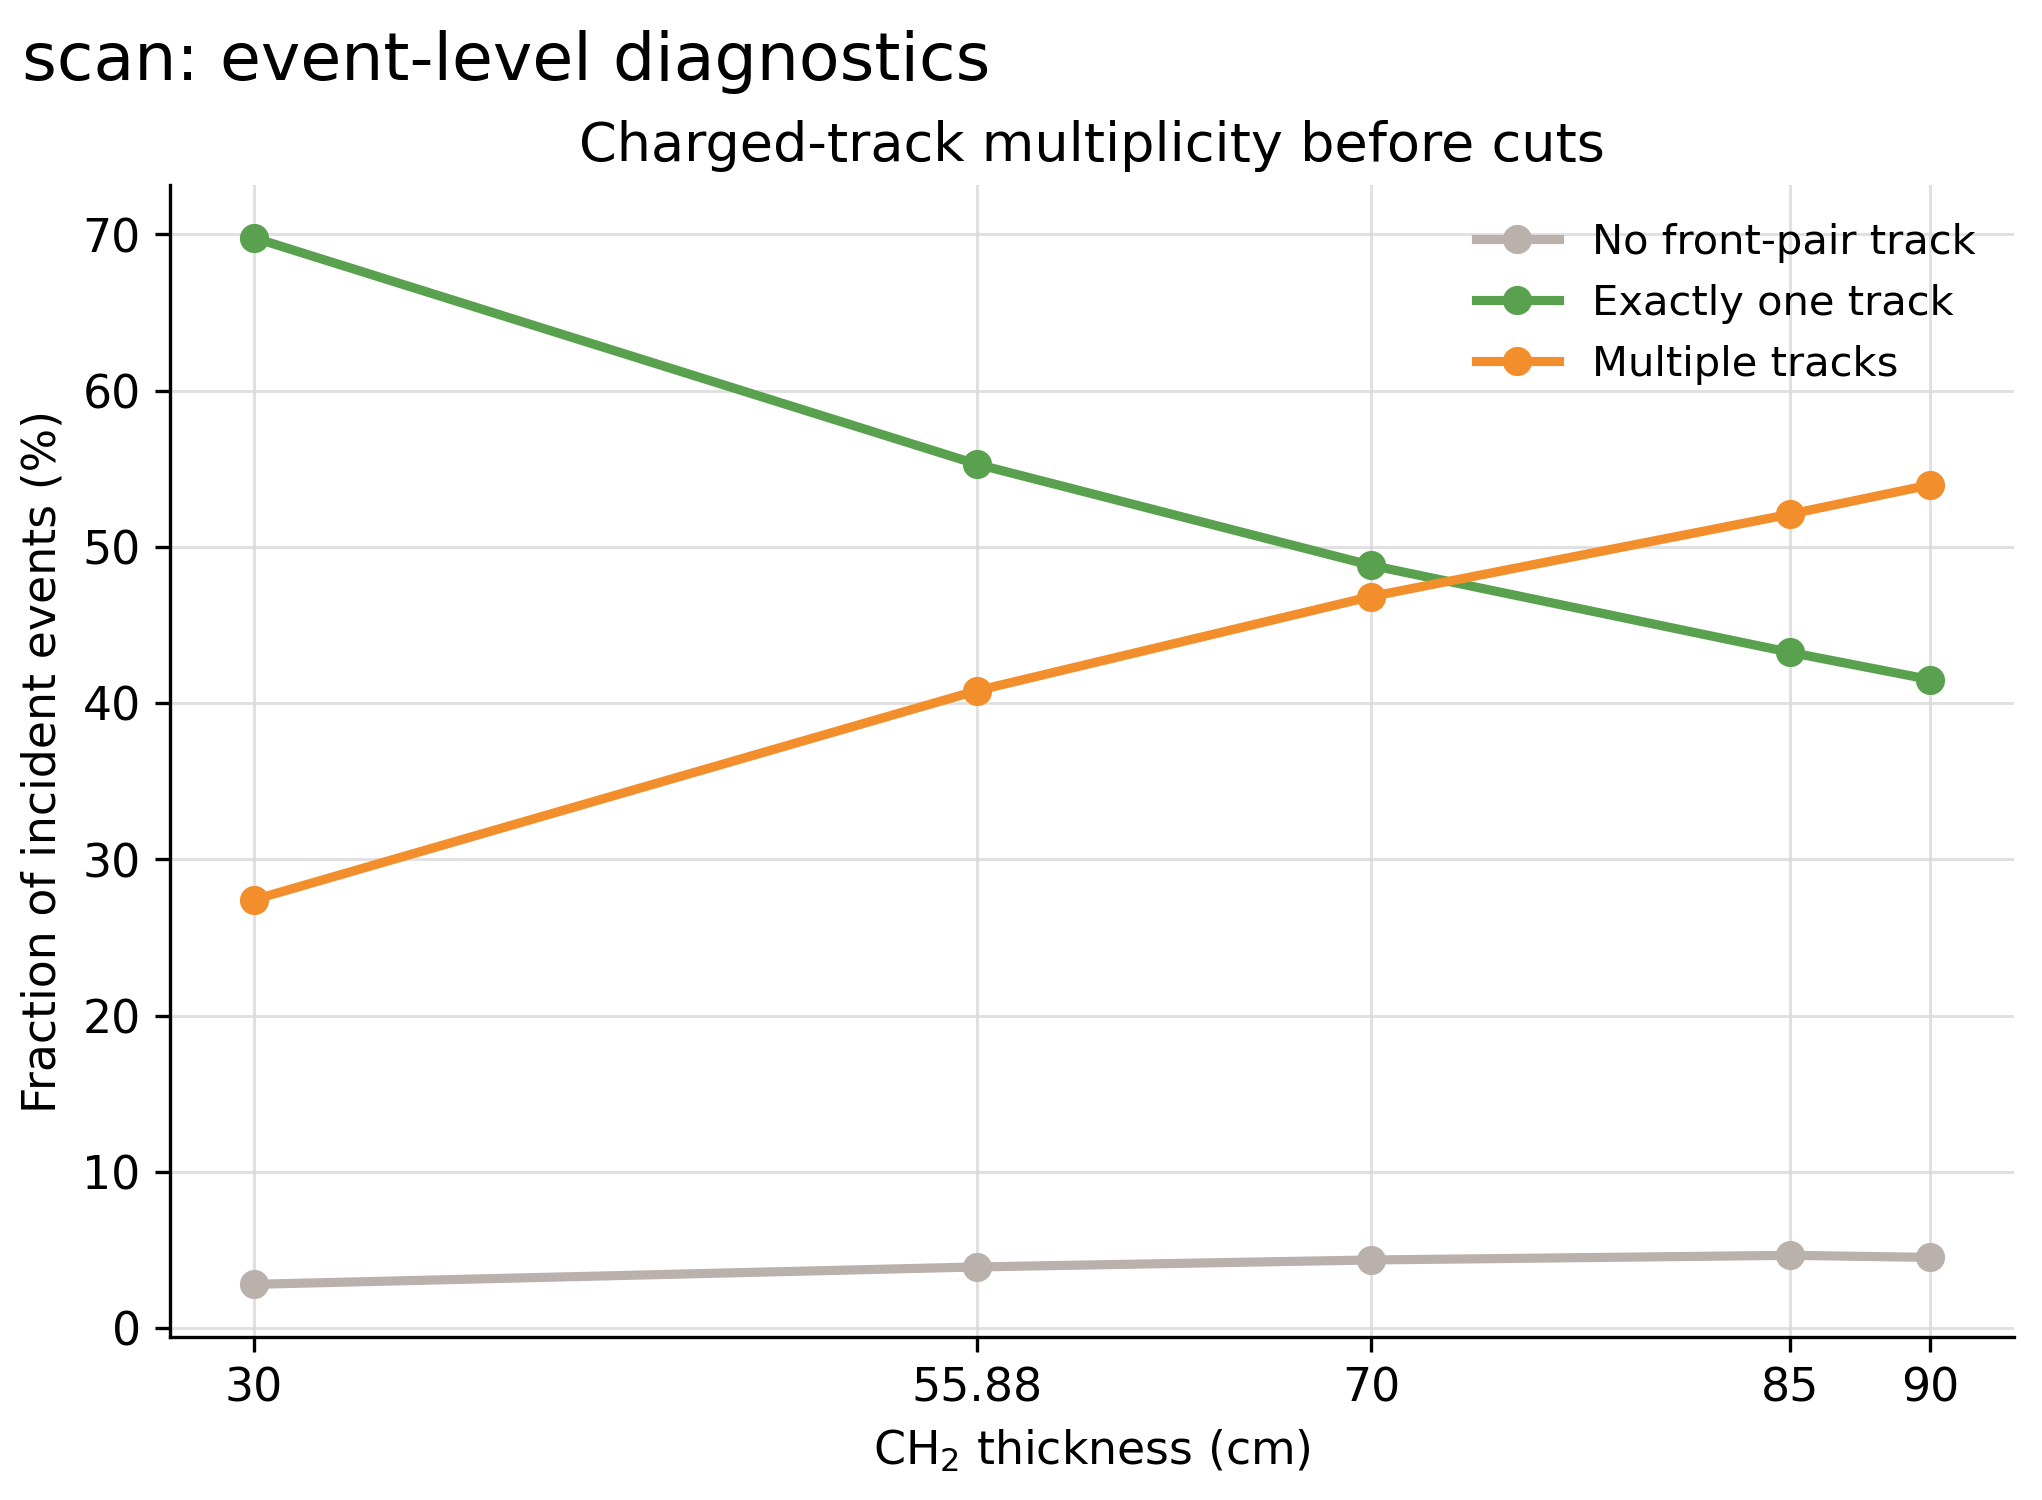
\includegraphics[width=\linewidth,height=0.57\textheight,keepaspectratio]{figures/thickness_multiplicity_panel_corrected.png}
    \end{column}
    \begin{column}{0.42\textwidth}
      \footnotesize
      \begin{block}{What is counted}
        Every charged candidate crossing both FPP1 and FPP2, before track
        ranking or any cone, closest-approach, angle, or $p_T$ cut.
      \end{block}
      Each curve uses the same denominator of 100,000 incident protons.
      \vspace{0.12cm}

      \textcolor{gray}{\textbf{Gray:}} no front-pair candidate.\\[3pt]
      \textcolor{green!60!black}{\textbf{Green:}} exactly one front-pair candidate.\\[3pt]
      \textcolor{orange}{\textbf{Orange:}} two or more front-pair candidates.

      \vspace{0.18cm}
      These three mutually exclusive categories sum to 100\% at each thickness.
    \end{column}
  \end{columns}
  \vspace{-0.05cm}
  \begin{block}{70 cm example}
    \footnotesize
    Gray: $4{,}358/100{,}000=4.358\%$. \quad
    Green: $48{,}820/100{,}000=48.820\%$.\\
    Orange: $46{,}822/100{,}000=46.822\%$. \quad
    Total: 100,000 events.
  \end{block}
  \note{Multiplicity is measured before the agreed selection chooses a track.
  A front-pair candidate need not cross FPP3 or FPP4 and need not pass the cone,
  z-close, s-close, angle, or useful-pT requirements. The selected-track yield
  on the preceding slide is therefore not a simple copy of the green or orange
  population.}
\end{frame}

% -----------------------------------------------------------------------------
\begin{frame}{Primary loss grows rapidly with analyzer thickness}
  \begin{center}
    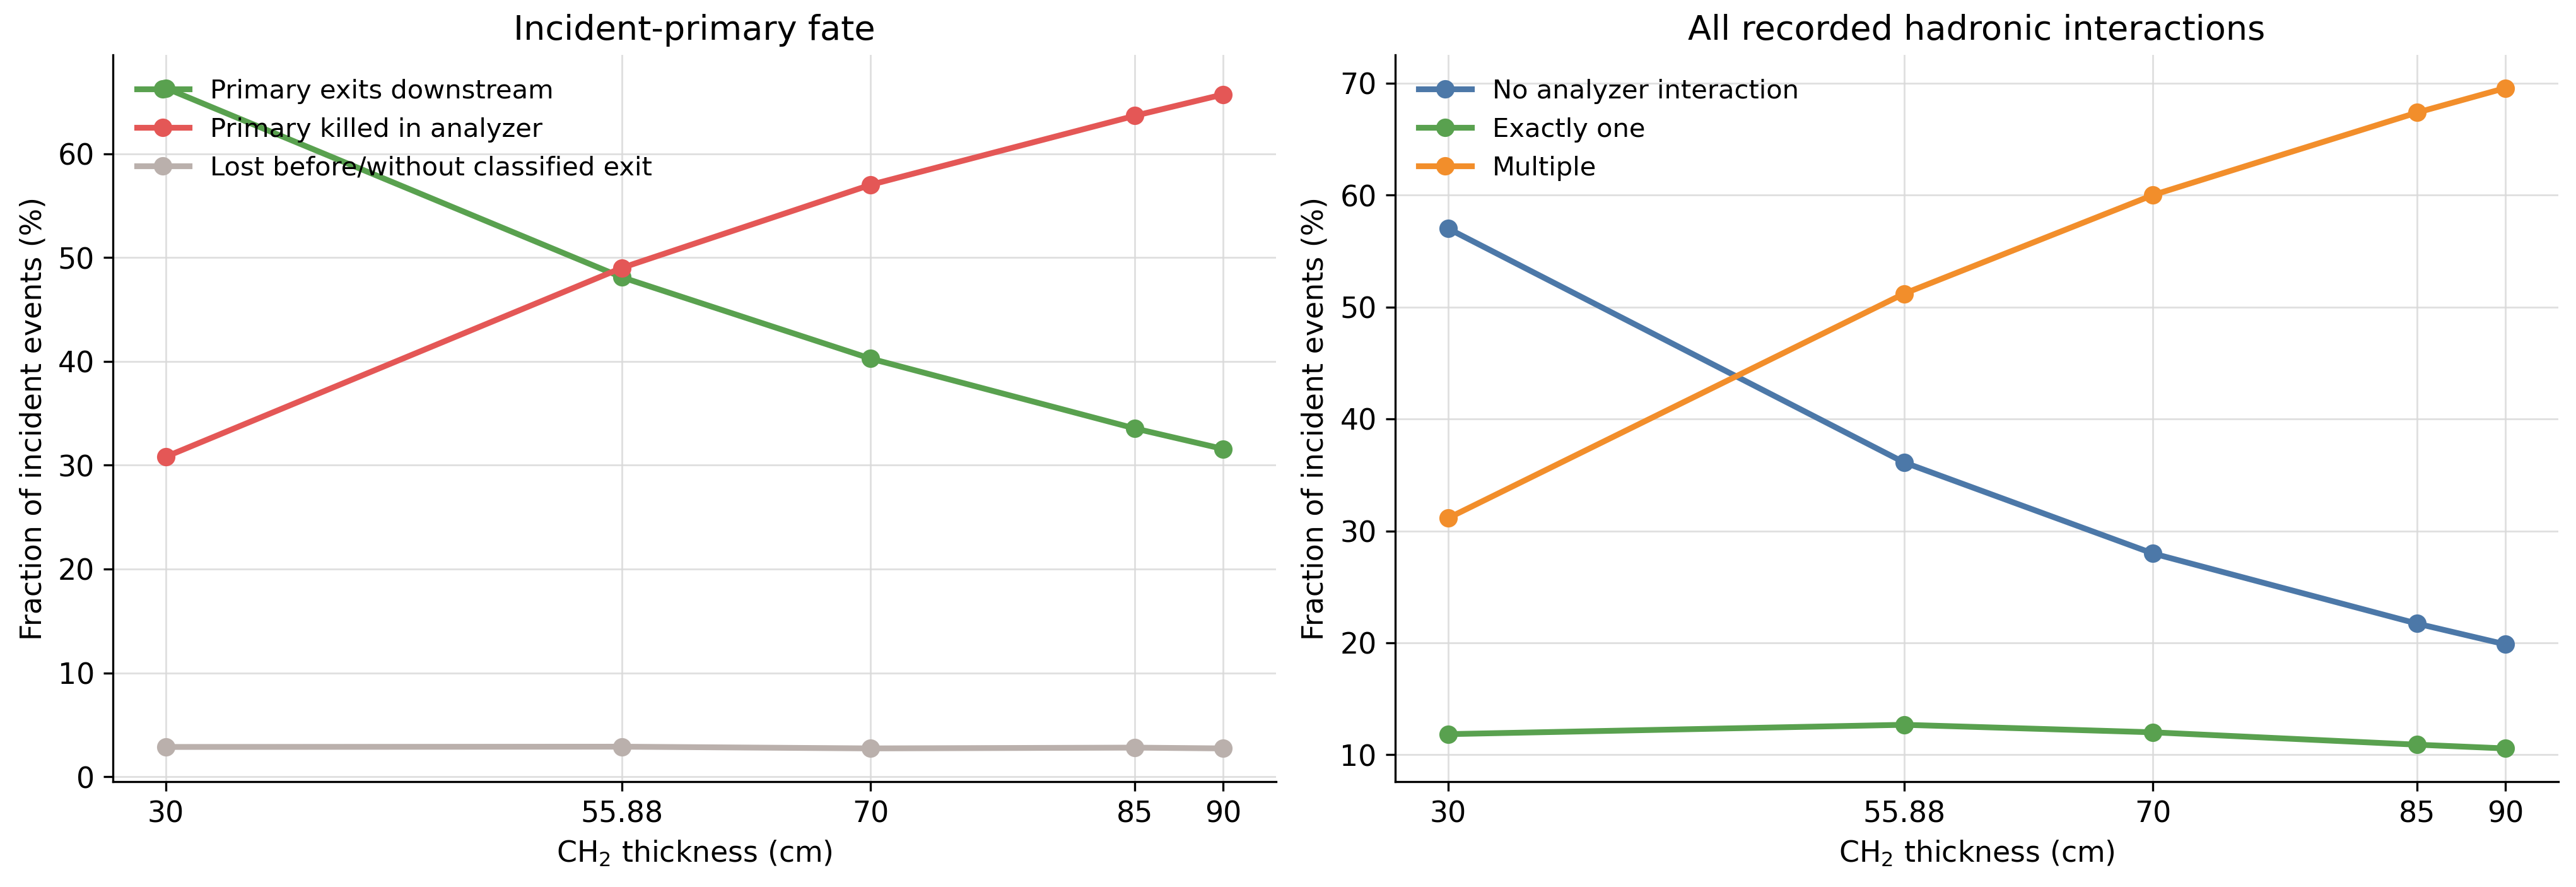
\includegraphics[width=0.98\linewidth,height=0.65\textheight,keepaspectratio]{figures/thickness_event_diagnostics_bottom_corrected.png}
  \end{center}
  \vspace{-0.18cm}
  \small
  \begin{itemize}
    \item The fraction of incident primaries killed in the analyzer grows from
      30.8\% at 30 cm to 65.7\% at 90 cm.
    \item Events with multiple recorded hadronic interactions grow from 31.1\%
      to 69.6\% over the same range.
    \item Added material initially creates more useful scattering. Beyond about
      70 cm, absorption and acceptance losses offset that gain.
  \end{itemize}
  \note{Primary-killed fractions are 30.815, 49.003, 57.005, 63.655, and
  65.703 percent. Multiple-interaction fractions are 31.137, 51.197, 60.004,
  67.379, and 69.564 percent. The simulation records every analyzer hadronic
  interaction, particle identity and charge, candidate lineage, and the
  incident-primary exit fate. The last bullet is an interpretation of the
  combined efficiency and fate diagnostics rather than a direct tag of a
  single loss mechanism.}
\end{frame}

% -----------------------------------------------------------------------------
\begin{frame}{Useful yield is dominated by secondary-inelastic tracks}
  \begin{center}
    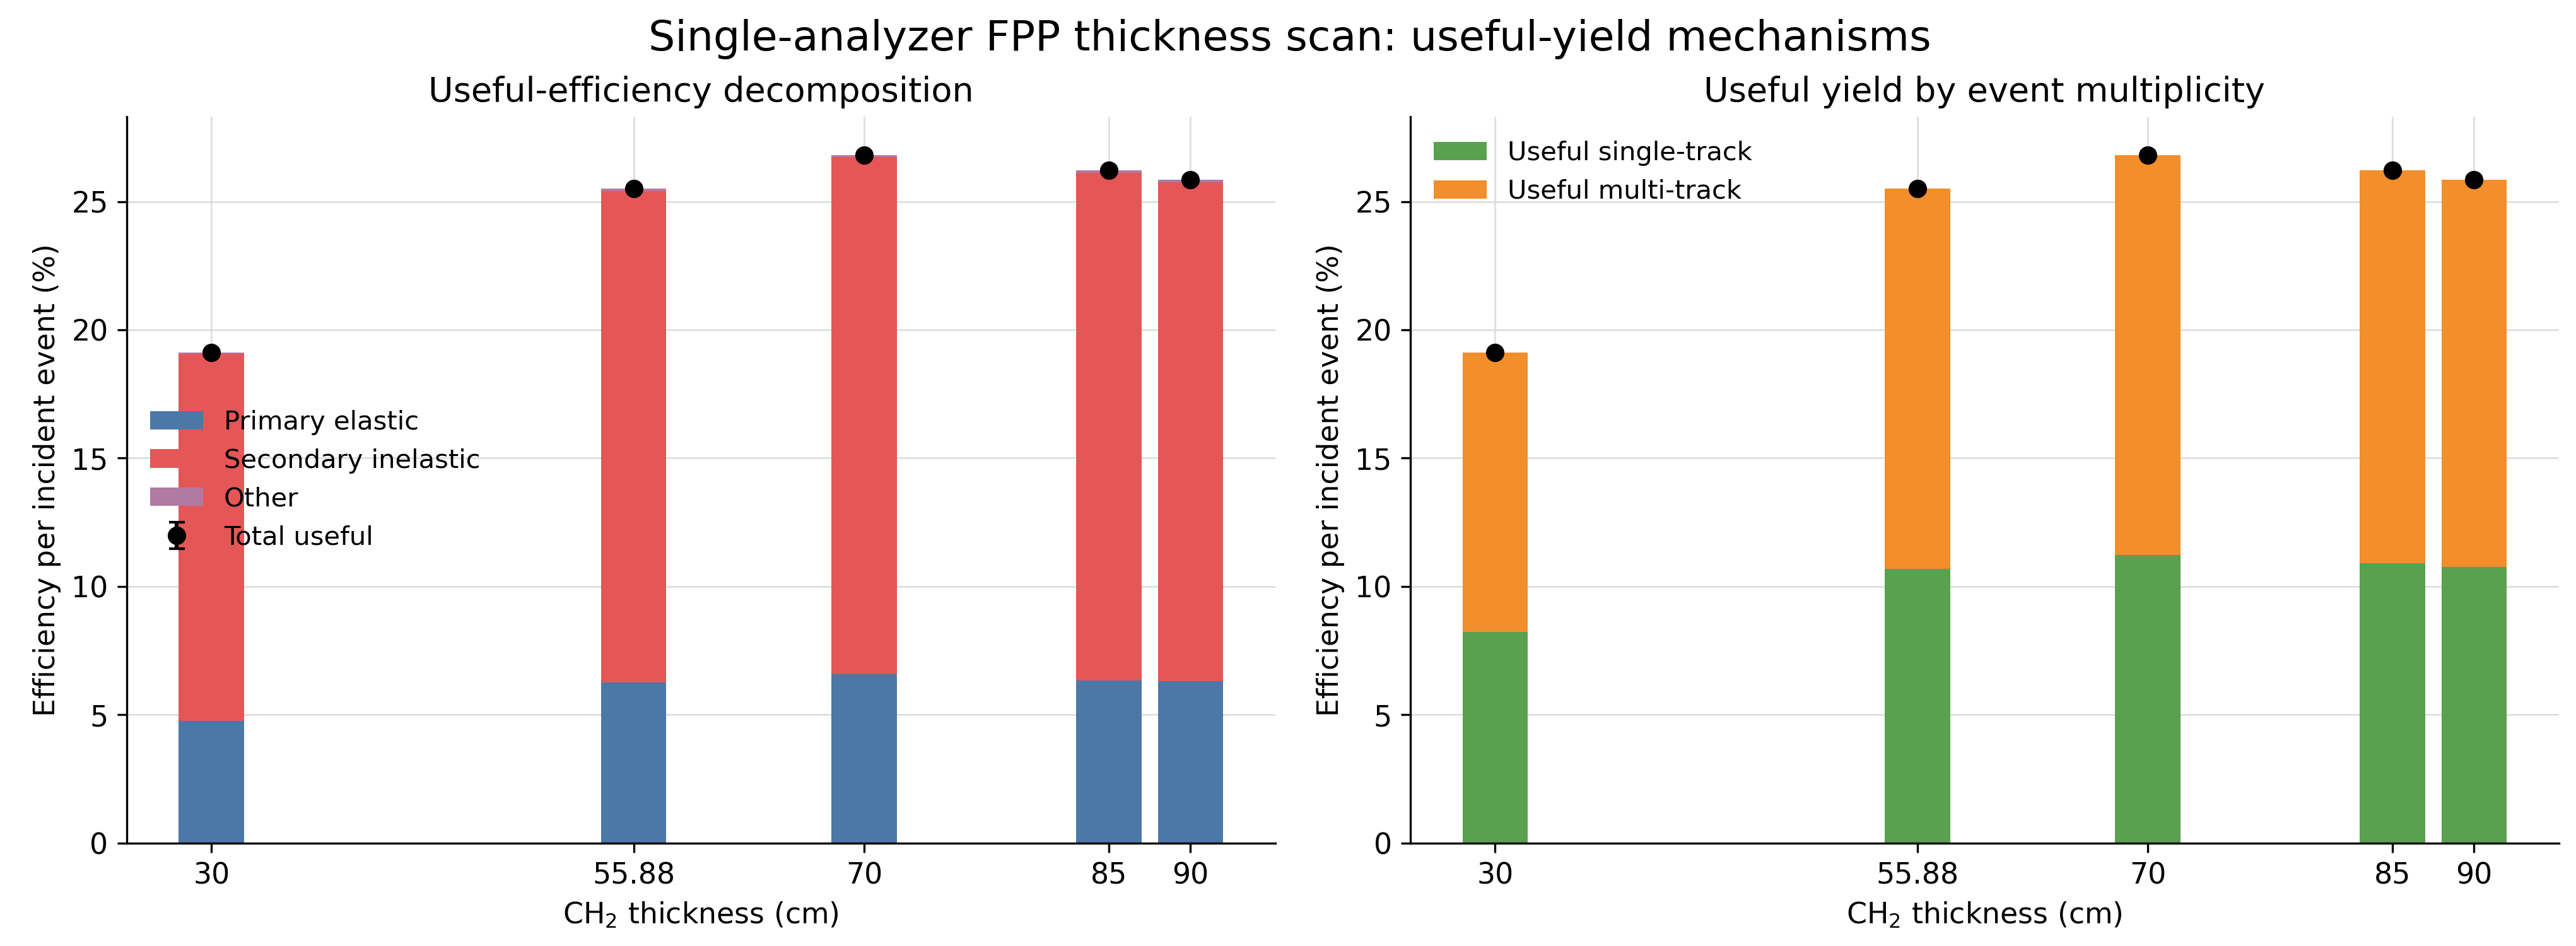
\includegraphics[width=0.98\linewidth,height=0.59\textheight,keepaspectratio]{figures/thickness_mechanism_decomposition_top_corrected.png}
  \end{center}
  \vspace{-0.18cm}
  \begin{block}{At the 70 cm maximum}
    \small
    The 26.81\% useful efficiency contains 6.59\% primary-elastic and 20.13\%
    secondary-inelastic contributions. Raw single-candidate and
    multiple-candidate events contribute 11.21\% and 15.60\%, respectively.
  \end{block}
  {\scriptsize The larger secondary-inelastic channel cannot inherit a
  single-proton analyzing-power model without dedicated validation.}
  \note{Primary-elastic useful efficiencies are 4.753, 6.264, 6.589, 6.325,
  and 6.300 percent. Secondary-inelastic useful efficiencies are 14.309,
  19.149, 20.134, 19.797, and 19.457 percent. Primary-inelastic and
  secondary-elastic contributions are essentially zero. Other contributions
  are below 0.1 percent. At 70 cm the useful single-candidate and
  multiple-candidate efficiencies are 11.212 and 15.598 percent. These classes
  refer to the raw front-pair multiplicity before selection.}
\end{frame}

% -----------------------------------------------------------------------------
\begin{frame}{Question 4: thickness-study assessment}
  \begin{center}
    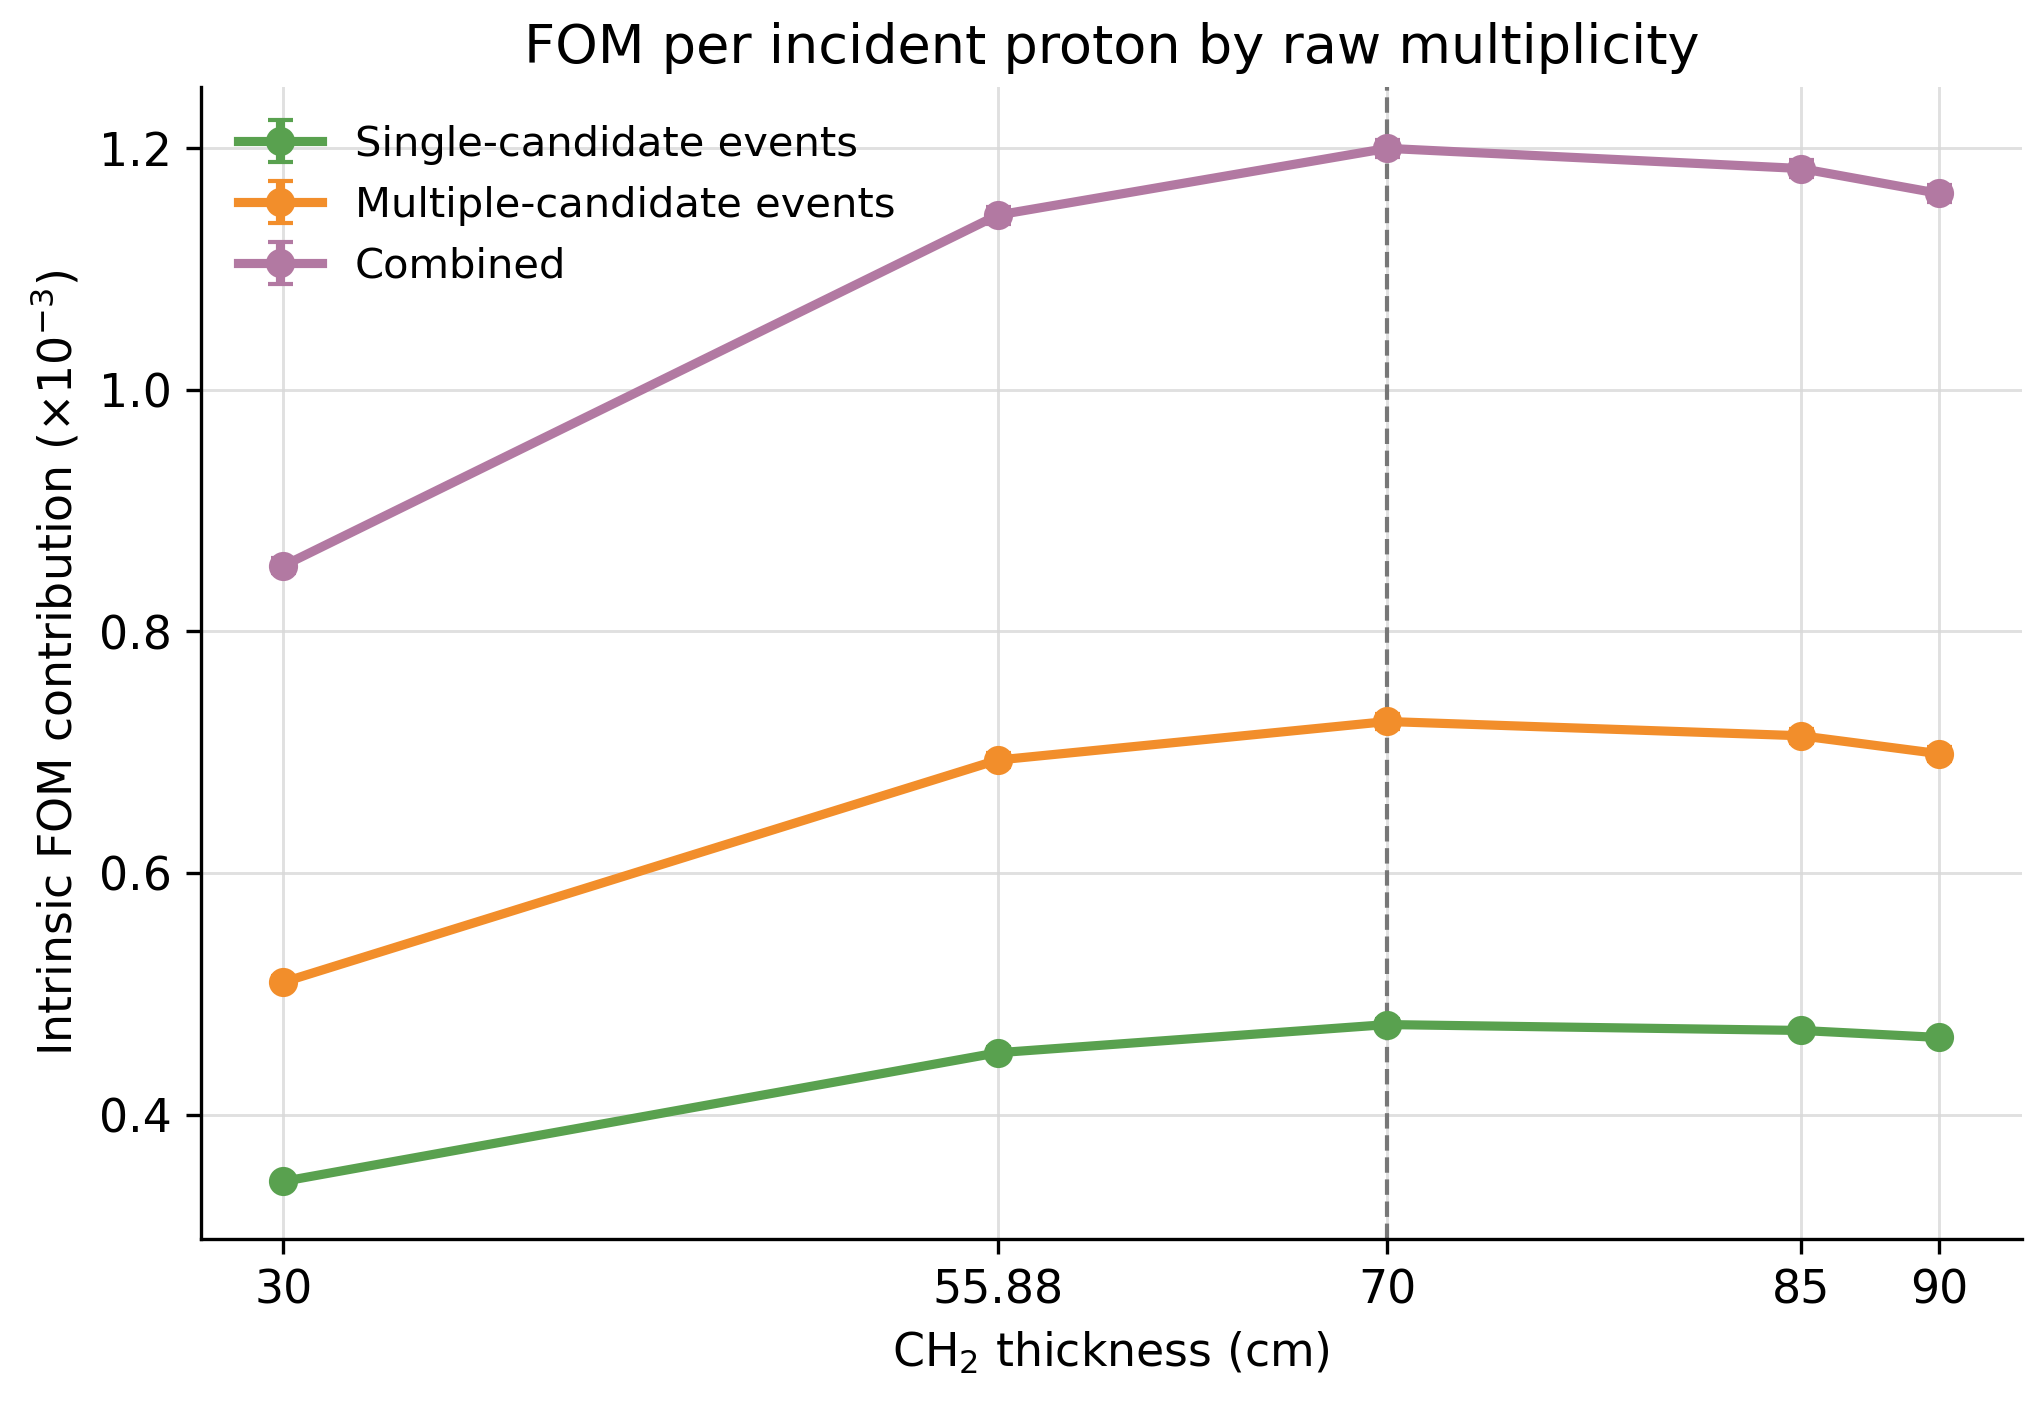
\includegraphics[width=0.88\linewidth,height=0.48\textheight,keepaspectratio]{figures/thickness_fom_panel_corrected.png}
  \end{center}
  \vspace{-0.18cm}
  \scriptsize
  \begin{itemize}
    \item Single-candidate, multiple-candidate, and combined FOM all have a
      broad maximum near 70 cm.
      Extending to 85--90 cm provides no statistical gain in this scan.
    \item At 70 cm, the intrinsic contributions per incident proton are
      $4.745\times10^{-4}$ from single-candidate events and
      $7.254\times10^{-4}$ from multiple-candidate events.
    \item Their sum is $1.200\times10^{-3}$. The multiple-candidate term remains
      provisional because it uses the GEp-III single-track $A_y$ model.
  \end{itemize}
  \vspace{-0.06cm}
  \begin{block}{Current answer}
    Mechanically plausible, but 70 cm is the next design point. Final choice
    requires channel-specific polarimetry and realistic reconstruction.
  \end{block}
  \note{The corrected combined intrinsic FOM values are 0.000854355,
  0.001144638, 0.001199898, 0.001183199, and 0.001162563 for 30, 55.88, 70,
  85, and 90 cm. At 70 cm, the single-candidate and multiple-candidate
  contributions are 0.000474496 and 0.000725402, which sum exactly to the
  combined value in the saved output.
  The 90 cm analyzer leaves about 26.3 cm to the assumed upstream face of the
  first FPP chamber structure in this compact layout. Reconstruction closure
  is excellent in the ideal simulation. The conclusion is therefore not that
  85--90 cm is geometrically impossible. It is that extra thickness does not
  improve the present physics metric and introduces substantially more event
  complexity.}
\end{frame}

\end{document}
